% Präambel
\documentclass[12pt,a4paper,oneside, 
liststotoc, 					% Tabellen- und Abbildungsverzeichnis ins Inhaltsverzeichnis
bibtotoc,						% Literaturverzeichnis ins Inhaltsverzeichnis aufnehmen
titlepage, 						% Titlepage-Umgebung statt \maketitle
headsepline, 					% horizontale Linie unter Kolumnentitel
%abstracton,					% Überschrift beim Abstract einschalten, Abstract muss dazu in {abstract}-Umgebung stehen
%DIV11,							% auskommentieren, um den Seitenspiegel zu vergrößern
BCOR10mm,						% Bindekorrektur, die den Seitenspiegel um 15mm nach rechts verschiebt,
]{scrreprt}			
\usepackage{ucs} 				% Dokument in utf8-Codierung schreiben und speichern
\usepackage[utf8x]{inputenc} 	% ermöglicht die direkte Eingabe von Umlauten
\usepackage[english, ngerman]{babel} 	% deutsche Trennungsregeln und Übersetzung der festcodierten Überschriften
\usepackage[T1]{fontenc} 		% Ausgabe aller zeichen in einer T1-Codierung (wichtig für die Ausgabe von Umlauten!)
\usepackage{graphicx}  			% Einbinden von Grafiken erlauben
%\usepackage{amsmath}
%\usepackage{amsfonts}
%\usepackage{amssymb}
\usepackage{mathpazo} 			% Einstellung der verwendeten Schriftarten
\usepackage{textcomp} 			% zum Einsatz von Eurozeichen u. a. Symbolen
\usepackage{listings}			% Datstellung von Quellcode mit den Umgebungen {lstlisting}, \lstinline und\lstinputlisting
\usepackage{xcolor} 			% einfache Verwendung von Farben in nahezu allen Farbmodellen
%\usepackage[intoc]{nomencl} 	% zur Erstellung des Abkürzungsberzeichnisses
\usepackage{fancyhdr}			% Zusatzpaket zur Gestaltung von Fuß und Kopfzeilen
\usepackage{jurabib}			% Paket für das Literaturverzeichniss
\usepackage{bibgerm}			% Deutsche Zitierweise
\usepackage[printonlyused]{acronym}
\usepackage{hyperref} 
\usepackage{float}
\usepackage{setspace}


%Zeilenumbrüche in URLs (besonders im Literaturverzeichnis)
\let\oldurlbraks=\UrlBreaks
\renewcommand{\UrlBreaks}{\oldurlbraks\do\a\do\b\do\c\do\d\do\e\do\f\do\g%
                           \do\h\do\i\do\j\do\k\do\l\do\m\do\n\do\o\do\p%
                           \do\q\do\r\do\s\do\t\do\u\do\v\do\w\do\x%
                           \do\y\do\z\do\?\do\&} 


% -----------------------------------------------------------------------------------------------------------------
% Zum Aktualisieren des Abkürzungsverzeichnisses bitte auf der Kommandozeile folgenden Befehl aufrufen :
%  makeindex Bachelorarbeit.nlo -s nomencl.ist -o Bachelorarbeit.nls
% -----------------------------------------------------------------------------------------------------------------

% Hier die persönlichen Daten eingeben:

\newcommand{\titel}{Optimierung des Shelf-Managements}
\newcommand{\titelzwei}{Shelf Management Augmented Reality}
\newcommand{\untertitel}{mit Hilfe von Augmented Reality auf Wearable-Computern}
\newcommand{\arbeit}{Große Studienarbeit}
\newcommand{\studiengang}{Angewandte Informatik Business Competence}
\newcommand{\autor}{Stephan Giesau, Sebastian Kowalski, Raffael Wojtas}
\newcommand{\matrikelnr}{5890600, 6664480, 7998056}
\newcommand{\kurs}{TINF12AI-BC}
\newcommand{\firma}{FIRMA?!}
\newcommand{\zeitraum}{12.05.2014 - 31.05.2015}
\newcommand{\betreuerdhbw}{Prof. Dr. Christian Buergy}
\newcommand{\betreuerfirma}{Max Mustermann}
\newcommand{\location}{Walldorf}

\newcommand{\jahr}{2015}			% für Angabe im Copyright-Vermerk der Titelseite

% Abkürzungen
\newcommand{\ua}{\mbox{u.\,a.\ }}
\newcommand{\zB}{\mbox{z.\,B.\ }}
\newcommand{\bs}{$\backslash$}
\newcommand{\bzw}{bzw. }

%\renewcommand{\nomname}{Abkürzungsverzeichnis}
\renewcommand{\baselinestretch}{1.5}

% -------------------------------------------------------------------------------------------
%                      Definition der Kopf- und Fußzeilen -------------------------------------------------------------------------------------------
\lhead{}								% Kopf links
\chead{}								% Kopf mitte
\rhead{\sffamily{\titelzwei}}				% Kopf rechts
\lfoot{}								% Fuß links
\cfoot{\sffamily{\thepage}}				% Fuß mitte
\rfoot{\sffamily{\autor}}				% Fuß rechts
\renewcommand{\headrulewidth}{0.4pt}	% Liniendicke Kopf
\renewcommand{\footrulewidth}{0.4pt}	% Liniendicke Fuß


%\makenomenclature							% Abkürzungsverzeichnis erstellen
%
% alle Abkürzungen, die in der Bachelorarbeit verwendet werden

\nomenclature{DHBW}{Duale Hochschule Baden-Württemberg}
\nomenclature{Sem}{Semester}
\nomenclature{OSS}{Open Source Software}					% Datei mit Abkürzungen laden
% -------------------------------------------------------------------------------------------
%                     Setup Literaturverzeichnis & Zitate -------------------------------------------------------------------------------------------

%\jurabibsetup{
%    commabeforerest,
%    ibidem=strict,
%    citefull=first,            %zitiert nur das erste Auftreten voll
%    see,
%    human,                    %Einstellungen für Geisteswissenschaftler   
%    titleformat={colonsep,all},
%}

\renewcommand{\bibnumberformat}[1]{[#1]}
\jurabibsetup{bibformat={numbered}}


\title=%5Crenewcommand">renewcommand*{\bibbtsep}{In: }
\title=%5Crenewcommand">renewcommand*{\bibjtsep}{In: }
\title=%5Crenewcommand">renewcommand*{\bibtfont}{\textit} 
\title=%5Crenewcommand">renewcommand*{\bibbtfont}{\textit}



% -------------------------------------------------------------------------------------------
%                     Beginn des Dokumenteninhalts -------------------------------------------------------------------------------------------
\begin{document}
\setcounter{secnumdepth}{3}					% Nummerierungstiefe fürs Inhaltsverzeichnis
\setcounter{tocdepth}{3}
%\setkomafont{sectioning}{\rmfamily} 
\sffamily									% für die Titelei serifenlose Schrift verwenden
\setlength{\parindent}{0pt}					% Einrückungen ausschalten

% -------------------------------------------------------------------------------------------
%                      Titelei -------------------------------------------------------------------------------------------
\setlength{\voffset}{-1cm}
\begin{spacing}{1}
	\thispagestyle{plain}
\begin{titlepage}
\enlargethispage{6.0cm}
\sffamily 								% Serifenlose Grundschrift für die Titelseite einstellen
				


			
				

%\includegraphics[scale=1.5]{Bilder/logo_SAP.png} 
\hfill

\includegraphics[scale=1.0]{Bilder/logo_dhbw_ma.jpg}\\[5ex] %5em


\begin{center}

\huge{\textsc{\textbf{\titel}}}\\[1.5ex]
\Large{\textbf{\untertitel}}\\[5ex]
\LARGE{\textbf{\arbeit}}\\[2ex]
\normalsize{des Studiengangs \studiengang~}\\[1ex]
\normalsize{an der Dualen Hochschule Baden-Württemberg Mannheim}\\[1ex]
von\\[1ex] 
\Large{\textbf{\autor}} \\[4ex] %18ex oder 10ex
\normalsize{September 2015} \\[16ex]

\end{center}

\begin{center} %flushleft

\begin{spacing}{1.3}
\begin{tabular}{ll}
\textbf{Bearbeitungszeitraum}:					& \quad\quad \zeitraum \\
\textbf{Matrikelnummern, Kurs}: 			& \quad\quad \matrikelnr , \kurs \\ 
% \textbf{Ausbildungsfirma}:	 			& \quad\quad \firma \\ 
% \textbf{Betreuer}:  & \quad\quad \betreuerfirma \\ 
\textbf{Wissenschaftlicher Betreuer}: & \quad\quad \betreuerdhbw \\ [5ex]

\end{tabular} 
\end{spacing}

\end{center}	%flushleft
\end{titlepage}
 				% erzeugt die Titelseite
\end{spacing}
\setlength{\voffset}{0cm}
\pagenumbering{Roman}						% große, römische Seitenzahlen für Titelei
% % Sperrvermerk bei Bedarf dekommentieren
%\hrule 
\chapter*{Sperrvermerk}
Die vorliegende Arbeit mit dem Titel {\itshape \titel - \untertitel} enthält vertrauliche Informationen der\\

\textbf{SAP SE\\
Dietmar-Hopp-Allee 16\\
69190 Walldorf}\\

Sie ist mit einem Sperrvermerk versehen und wird ausschließlich zu Prüfungszwecken für {\studiengang} der Dualen Hochschule Baden-Württemberg Mannheim vorgelegt.\\
Jede Einsichtnahme und Veröffentlichung – auch von Teilen der Arbeit – bedarf der vorherigen Zustimmung durch die {\firma}.


%\newpage
%
%
%\addchap*{Erklärung}
%gemäß § 5 (3) der \glqq Studien- und Prüfungsordnung DHBW Technik\grqq vom 22. September 2011.
%Ich habe die vorliegende Arbeit selbstständig verfasst und keine anderen als die angegebenen Quellen und Hilfsmittel verwendet.\\
%
%%Ich versichere hiermit, dass ich meine \arbeit~ mit dem Thema
%%\begin{quote}
%%\textit{\titel} -\textit{ \untertitel }
%%\end{quote}
%%selbständig verfasst und keine anderen als die angegebenen Quellen und Hilfsmittel benutzt habe. Die Arbeit wurde bisher keiner anderen Prüfungsbehörde vorgelegt und auch nicht veröffentlicht.\\
%
%%Mir ist bekannt, dass ich meine \arbeit zusammen mit dieser Erklärung fristgemäß nach Vergabe des Themas in doppelter Ausfertigung und gebunden im Sekretariat meines Studiengangs an der DHBW Mannheim abzugeben habe. Als Abgabetermin gilt bei postalischer Übersendung der Eingangsstempel der DHBW, also nicht der Poststempel oder der Zeitpunkt eines
%%Einwurfs in einen Briefkasten der DHBW.\\[10ex]
%
%\location, \today \\[4ex]
%\rule[-0.2cm]{5cm}{0.5pt} \\
%\textsc{\autor} \\[10ex]














% Sperrvermerk bei Bedarf dekommentieren
%\hrule 
\chapter*{Erklärung}
gemäß § 5 (3) der \glqq Studien- und Prüfungsordnung DHBW Technik\grqq~ vom 22. September 2011.
Wir haben die vorliegende Arbeit selbstständig verfasst und keine anderen als die angegebenen Quellen und Hilfsmittel verwendet.\\

\location, \today \\[4ex]
\rule[-0.2cm]{5cm}{0.5pt} \\
\textsc{\autor} \\[10ex]


%
%%Ich versichere hiermit, dass ich meine \arbeit~ mit dem Thema
%%\begin{quote}
%%\textit{\titel} -\textit{ \untertitel }
%%\end{quote}
%%selbständig verfasst und keine anderen als die angegebenen Quellen und Hilfsmittel benutzt habe. Die Arbeit wurde bisher keiner anderen Prüfungsbehörde vorgelegt und auch nicht veröffentlicht.\\
%
%%Mir ist bekannt, dass ich meine \arbeit zusammen mit dieser Erklärung fristgemäß nach Vergabe des Themas in doppelter Ausfertigung und gebunden im Sekretariat meines Studiengangs an der DHBW Mannheim abzugeben habe. Als Abgabetermin gilt bei postalischer Übersendung der Eingangsstempel der DHBW, also nicht der Poststempel oder der Zeitpunkt eines
%%Einwurfs in einen Briefkasten der DHBW.\\[10ex]
%














 				% Einbinden der eidestattlichen Erklärung
\chapter*{Abstract} %*-Variante sorgt dafür, das Abstract nicht im Inhaltsverzeichnis auftaucht
\sloppy
Die folgende Arbeit beschäftigt sich mit der Optimierung des \glqq Shelf-Managements\grqq~im Einzelhandel. Dabei wurde versucht, veraltete und historisch gewachsene Verfahren durch neue Prozesse, die durch \glqq Wearable-Computern\grqq~unterstützt werden, abzulösen.\\

Ziel dieser Arbeit ist das Entwickeln einer Gesamtlösung, bestehend aus einer Administrationsoberfläche zur Bestands-/Regal-/Produktverwaltung und einer Android App, die sämtliches Papier während der Warenannahme und -einräumung ablösen soll. Diese Lösung soll als \glqq Proof of Concept\grqq~verstanden werden und die nötige Flexibilität für Live-Demos in kleineren Filialen mitbringen.\\

Externe durchgeführte Studien, sowie eine im Rahmen dieses Projektes durchgeführte Umfrage bei Filialleitern einer Supermarktkette\footnote{Name aus datenschutzrechtlichen Gründen nicht genannt.} stellen die aktuellen Probleme beim Shelf-Management im Einzelhandel dar. Darüber hinaus stellen diese Informationen die Grundlage für die durchgeführte Bedarfs- und Anforderungsanalyse dar. Auf Grundlage der Anforderungen wird die Architektur entwickelt.\\

Die Konzepte der Implementierung sowie die verwendete Technik werden detailliert erklärt, um eine Weiterentwicklung und Fortführung dieses Projektes zu ermöglichen.\\

Alle definierten Ziele der ersten Priorität wurden im gegebenen Zeitrahmen erfüllt und bilden die Grundlage für einen erfolgreichen \glqq Proof of Concept\grqq . Da ein Testen der Anwendung in realem Umfeld im Rahmen dieser Arbeit nicht möglich war, können eventuell auftretende Schwächen und falsch interpretierte Anforderungen nicht herausgestellt werden. Die Anwendung benötigt daher weitere Entwicklungszeit und Analyse während der ersten Tests. Darüber hinaus fallen bereits während der Entwicklung Schwachstellen in der zur Verfügung stehenden Technik auf: das Display der Smartglass wirkt undeutlich und erschwert das Ablesen der nötigen Informationen.\\

Das Projekt ist im Rahmen der gestellten Ziele ein Erfolg und zeigt die Möglichkeiten und Chancen auf, die sich durch ein computergestütztes Shelf-Management ergeben.
\fussy   				% Einbinden des Abstracts
% \chapter*{Formular der Aufgabenstellung} %*-Variante sorgt dafür, das Abstract nicht im Inhaltsverzeichnis auftaucht


\begin{spacing}{1.3}
\begin{tabular}{ll}
\underline{\textbf{Studentin/Student}}	& \\
\textbf{Kurs [TINFxyAI-XY]}: 			& \quad \kurs \\ 
\textbf{Studienjahr [1, 2, 3]}:			& \quad	3\\
\textbf{Praxiseinsatz [1, 2, 3, 4, 5, 6]}:	& \quad 5\\
\textbf{Name, Nachname}:				& \quad Marx, Miriam\\
\textbf{Unternehmen}:	 				& \quad \firma \\ 
\textbf{Tel.-Nummer}: 					& \quad  +49 6227 7-79806\\ 
\textbf{E-Mail-Adresse}: 				& \quad miriam.marx@sap.com  \\ [2ex]
%\end{tabular} 
%\end{spacing}

%\begin{spacing}{1.3}
%\begin{tabular}{ll}
\underline{\textbf{Betreuerin/Betreuer}}	& \\
\textbf{Name, Nachname}: 				& \quad \betreuerfirma \\ 
\textbf{Unternehmen}:					& \quad	SAP SE\\
\textbf{Abteilung}:						& \quad Abteilung XY\\
\textbf{Akad. Grad / Position}:			& \quad Dr. rer. nat./ Senior Director\\
\textbf{Tel.-Nummer}:	 				& \quad +49 0000000000 \\ 
\textbf{E-Mail-Adresse}: 				& \quad max.mustermann@sap.com  \\ [6ex]
\end{tabular} 
\end{spacing}


\textbf{Titel der Praxisarbeit}\\
\titel\\

\textbf{Kurzbeschreibung der Praxisarbeit}\\
Lorem ipsum dolor sit amet, consetetur sadipscing elitr, sed diam nonumy eirmod tempor invidunt ut labore et dolore magna aliquyam erat, sed diam voluptua. At vero eos et accusam et justo duo dolores et ea rebum. Stet clita kasd gubergren, no sea takimata sanctus est Lorem ipsum dolor sit amet. Lorem ipsum dolor sit amet, consetetur sadipscing elitr, sed diam nonumy eirmod tempor invidunt ut labore et dolore magna aliquyam erat, sed diam voluptua. At vero eos et accusam et justo duo dolores et ea rebum. Stet clita kasd gubergren, no sea takimata sanctus est Lorem ipsum dolor sit amet.\\


\textbf{Geplante Vorgehensweise während der Praxisphase}\\
Lorem ipsum dolor sit amet, consetetur sadipscing elitr, sed diam nonumy eirmod tempor invidunt ut labore et dolore magna aliquyam erat, sed diam voluptua. At vero eos et accusam et justo duo dolores et ea rebum. Stet clita kasd gubergren, no sea takimata sanctus est Lorem ipsum dolor sit amet. Lorem ipsum dolor sit amet, consetetur sadipscing elitr, sed diam nonumy eirmod tempor invidunt ut labore et dolore magna aliquyam erat, sed diam voluptua. At vero eos et accusam et justo duo dolores et ea rebum. Stet clita kasd gubergren, no sea takimata sanctus est Lorem ipsum dolor sit amet.\\

Lorem ipsum dolor sit amet, consetetur sadipscing elitr, sed diam nonumy eirmod tempor invidunt ut labore et dolore magna aliquyam erat, sed diam voluptua. At vero eos et accusam et justo duo dolores et ea rebum. Stet clita kasd gubergren, no sea takimata sanctus est Lorem ipsum dolor sit amet. Lorem ipsum dolor sit amet, consetetur sadipscing elitr, sed diam nonumy eirmod tempor invidunt ut labore et dolore magna aliquyam erat, sed diam voluptua. At vero eos et accusam et justo duo dolores et ea rebum. Stet clita kasd gubergren, no sea takimata sanctus est Lorem ipsum dolor sit amet.\\


	% Einbinden des Formulars der Aufgabenstellung

\tableofcontents							% Erzeugen des Inhalsverzeichnisses
%\printnomenclature[2.0cm]					% Erzeugen des Abkürzungsverzeichnisses
\newpage
%\pagestyle{empty}
%\begin{document}

\newcommand{\acronymname}{Abkürzungsverzeichnis}
%\chapter{Acronym}
\section*{\huge{Abkürzungsverzeichnis}}

\begin{acronym}
\setlength{\itemsep}{-\parsep}

\acro{3D}{drei Dimensionen}
\acro{AJAX}{Asynchronous JavaScript and XML}
\acro{API}{Application Programming Interface}
\acro{AR}{Augmented Reality}
\acro{AuthN}{Authentifizierung}
\acro{AuthZ}{Autorisierung}
\acro{BDSG}{Bundesdatenschutzgesetz}
\acro{cm}{Zentimeter}
\acro{CMS}{Content Management System}
\acro{CSS}{Cascading Style Sheets}
\acro{DBMS}{Datenbankmanagementsystem}
\acro{GB}{Gigabyte}
\acro{GHz}{Gigahertz}
\acro{HTML}{Hypertext Markup Language}
\acro{HTTP}{HyperText Transfer Protocol}
\acro{JWT}{JSON Web Token}
\acro{JS}{JavaScript}
\acro{JSON}{JavaScript Object Notation}
\acro{MAC}{Media-Access-Control}
\acro{MHz}{Megahertz}
\acro{PHP}{PHP Hypertext Preprocessor}
\acro{REST}{Representational State Transfer}
\acro{SMAR}{Shelf Management Augmented Reality}
\acro{SQL}{Structured Query Language}
\acro{SVG}{Scalable Vector Graphic}
\acro{USB}{Universal Serial Bus}
\acro{VR}{Virtual Reality}
\acro{WEP}{Wired Equivalent Privacy}
\acro{WLAN}{Wireless Local Area Network}
\acro{XML}{eXtensible Markup Language}





\acro{CAS}{Children's Aid Society}

\acro{OLTP}{Online Transaction Processing}

\acro{OLAP}{Online Analytical Processing}

\acro{DXC}{Direct Extractor Connection}

\acro{INA}{Information Access}

\acro{MMP}{Massive Parallel Processing}

\acro{RAM}{Random Access Memory}

\acro{CPU}{Central Processing Unit}



\acro{CSIS}{Child Success Information System}

\acro{ECW}{E-Clinical Works}

\acro{EHS}{Early Head Start}

\acro{ESL}{English as a second language}

\end{acronym}


\addcontentsline{toc}{chapter}{Acronym}
\newpage
\listoffigures 								% Erzeugen des Abbildungsverzeichnisses 
%\lstlistoflistings 							% Erzeugen des Quellcodeverzeichniss
\pagebreak



% ------------------------------------------------------------------------------------------- 
%                      Listings -------------------------------------------------------------------------------------------
\makeatletter
\renewcommand*{\lstlistoflistings}{%
  \begingroup
    \if@twocolumn
      \@restonecoltrue\onecolumn
    \else
      \@restonecolfalse
    \fi
    \lol@heading
    \setlength{\parskip}{\z@}%
    \setlength{\parindent}{\z@}%
    \setlength{\parfillskip}{\z@ \@plus 1fil}%
    \@starttoc{lol}%
    \if@restonecol\twocolumn\fi
  \endgroup
}
\makeatother

%Settings ABAP
\lstset{language=[R/3 6.10]ABAP}		
\lstset{morecomment=[f][commentstyle][0]*}
\lstset{captionpos=b}
\lstset{numbers=left}
\lstset{numberstyle=\small}
\lstset{numbersep=10pt}
\lstset{keywordstyle=\bfseries\color{violet}}
\lstset{commentstyle=\color{red}}
\lstset{stringstyle=\itshape\color{darkgray}}
\lstset{showstringspaces=false} 
\lstset{frame=single}
\lstset{framexleftmargin=8mm}
\lstset{breaklines=true}
\lstset{lineskip={-4.0pt}}
% ----------------------------------------------------------------------------------------------
%                    Inhalt der Bachelorarbeit
%---------------------------------------------------------------------------------------------
\pagenumbering{arabic}						% arabische Seitenzahlen für den Hauptteil
\pagestyle{fancy}					
\rmfamily

\chapter{Bedarfsanalyse}
\label{cha:bedarfsanalyse}
In diesem Kapitel sollen die grundlegenden Prozesse des Shelf-Managements näher betrachtet werden. Dazu werden die Prozesse der Warenannahme, des Einräumens von Waren und der Kundenservice in einem Einzelhandel beispielhaft und ohne technische Unterstützung dargestellt, analysiert und anschließend Problemstellen aufgezeigt. Dabei wird insbesondere auf die Schwachstellen und Verbesserungspotenzial eingegangen.\\
Anschließend werden aus den Problemen und Schwachstellen Ziele definiert, die im weiteren Verlauf der Arbeit weiter analysiert und schließlich durch technologische Unterstützung erfüllt werden sollen.

\section{Warenannahme}
\label{cha:warenannahme}
Damit überhaupt Produkte in Regale eingeräumt werden können, muss die Ware zunächst in das Geschäft gelangen. Zunächst werden Waren durch geschultes Personal bestellt und anschließend nach einer gewissen Zeit von einem Transporter angeliefert. Die Waren werden üblicherweise auf Paletten verpackt, ein Lieferschein ist beigelegt. Sofern Ware bestellt und geliefert wurde, muss die Ware abgenommen werden. \glqq Abnehmen\grqq bedeutet in diesem Kontext, dass die Ware von der Filiale offiziell als geliefert gekennzeichnet wurde. Dazu gehört das Zählen der gelieferten Ware und der Abgleich mit den Positionen der Bestellung; hier wird überprüft, ob die Menge der bestellten Ware mit der gelieferten Menge übereinstimmt. Dazu wird eine sogenannte Setzliste verwendet, welche eine Kopie der Bestellung ist. Die Setzliste ist dabei nicht mit dem Lieferschein zu verwechseln.\\

Wurde die Palette abgearbeitet und die Setzliste abgehakt bzw. Differenzen zwischen Lieferung und Bestellung angegeben, wird diese zu einer Führungskraft des Geschäfts gebracht, damit diese die Setzliste offiziell unterzeichnet und dann in ein elektronisches System überträgt. Nach diesem Arbeitsschritt ist es möglich, in der Buchhaltung die entsprechenden Beträge zu verbuchen.\\

Solange die Ware nicht im Verkaufsraum benötigt wird, wird diese im Lager des Geschäfts aufbewahrt. Dieser Prozess ist in folgendem Aktivitätsdiagramm visualisiert und zeigt mögliche Fehlerquellen, Risiken und Problemstellen. Diese Erkenntnisse sind mithilfe von erfahrenen und sehr geschulten Führungskräften von einem führenden Einzelhändler in der eingangs erwähnten Studie erarbeitet worden.\\

%TODO
[Aktivitätsdiagramm einfügen]\\

Wie in der Abbildung ersichtlich, fängt der Prozess bei der Bestellung von Waren an. Das verantwortliche Personal muss ohne technische Hilfsmittel selbst einschätzen können, welche Waren zum jeweiligen Zeitpunkt benötigt werden und in welchen Mengen diese Waren bestellt werden sollen. Dabei spielen verschiedene Aspekte eine große Rolle, etwa der Wochentag der Bestellung, das Wetter, die Jahreszeit, oder ob momentan Schulferien sind -- also alle Faktoren, die den Absatz einer Ware beeinflussen können. Beispielsweise ist während der Schulzeit die Käufergruppe der Schüler stärker vertreten als während der Ferienzeit, sodass bestimmte Waren stärker oder weniger nachgefragt werden.\\
Folglich ist es nur wenigen, erfahrenen Mitarbeitern möglich, eine sinnvolle Bestellung durchzuführen. Es ist allerdings wünschenswert, dass möglichst viele Mitarbeiter schnell bestellen können, sodass man unabhängiger von bestimmten Personen vor Ort wird, aber dennoch sorgfältige und sinnvolle Bestellungen tätigt.\\

Der Schritt \glqq Ware abnehmen\grqq erfordert die angesprochene Setzliste, welche auf Papier vorliegt. Dabei ist anzumerken, dass der Mitarbeiter durch das Abhaken der Setzliste keine Hand frei hat. Es wäre jedoch vorteilhaft, wenn der Mitarbeiter die Hände frei zum Arbeiten an der Palette hätte, um die Waren zu zählen. Außerdem können Fehler bei Bearbeitung der Setzliste geschehen, wie \zB ein Verzählen des Mitarbeiters. Zusätzlich sollte sofort bei Anlieferung die Ware überprüft werden, um die direkte Zuordnung zur Setzliste zu erhalten. So wird auch ein möglicher, unnötiger Verlust oder Beschädigung der Liste, und somit weitere Arbeit vermieden.\\
Angenommen, die Erfassung der Waren bei der Warenannahme würde durch eine entsprechende elektronische Lösung ersetzt, hätte der Mitarbeiter eine oder beide Hände immer frei zum Arbeiten. Da der Mitarbeiter, bei entsprechend automatisierter Warenerfassung, nicht mehr selbst zählen und vergleichen muss, ist die Fehlerwahrscheinlichkeit geringer als bei einer manuellen Erfassung und verspricht korrektere Buchungen sowie im Anschluss genauere Analysen. Außerdem ist es grundsätzlich schwieriger, eine elektronisch gespeicherte Liste zu verlieren.\\

Der nächste Arbeitsschritt, \glqq Ware in Lager einräumen\grqq , kostet in der Regel kaum Zeit, auch wenn er durch unerfahrenes Personal durchgeführt wird. Allerdings geht durch einen hohen Warenbestand im Lager viel Platz verloren, der im Idealfall besser genutzt werden könnte –- nämlich zum Verkauf von weiterer Ware, indem die Lagerfläche reduziert wird. Platz ist eine kostbare Ressource, wie man zum Beispiel an Grundstückspreisen feststellen kann. Außerdem besteht bei größerer Verkaufsfläche mehr Potential, den Umsatz zu erhöhen. Bei angemessenen Bestellungen und korrekten Lieferungen wird Ware sofort auf die Verkaufsfläche gestellt, sodass sie, im besten Fall, gar nicht erst im Lager aufbewahrt wird.\\

Wenn eine materielle Setzliste durch ein elektronisches Pendant abgelöst würde, entfielen Arbeitsprozesse wie \glqq Setzliste ins Büro bringen\grqq oder \glqq Setzliste mit abgenommener Ware vergleichen\grqq, sodass auch weiterer Mehraufwand durch verlorene oder falsche Lieferungen eingespart würde. Dabei ist anzumerken, dass der Aufwand bei falscher Lieferung zunächst nur in der Filiale entfällt. Die übergeordnete Instanz, die sich um die filialspezifischen Buchungen kümmert, muss dennoch die (Falsch-)Buchungen weiter arbeiten. Allerdings sind so die Daten schon von Beginn an digital erfasst und können ohne zusätzliches manuelles Eingreifen direkt weiter verarbeitet werden.

\section{Waren einräumen}
\label{waren_einräumen}
Während der Prozess der Warenannahme sich darauf beschränkt, die Ware vom Lieferanten entgegen zu nehmen und korrekt zu dokumentieren, behandelt das Shelf-Management das eigentliche Einräumen der Produkte in die Regale auf der Verkaufsfläche.\\

Ein Mitarbeiter muss die Ware aus dem Lager heraus an die richtige Stelle in den Regalen einräumen, und dies möglichst schnell, da sonst verderbliche Ware (wie \zB tiefgekühlte Lebensmittel) an Qualität verliert und insbesondere potenzieller Umsatz verloren geht, wenn Ware im Regal nicht vorrätig ist. Der Mitarbeiter nimmt die einzuräumende Ware im Normalfall auf einer Palette oder einem vergleichbar großen Container mit auf die Verkaufsfläche und stellt diese im Gang am Regal ab, um die Waren einzuräumen. Dabei steht er Kunden im Weg, die sich häufig über die Behinderung während des Einkaufs ärgern. Dies ist aus der Eingangs erwähnten Studie bei einem Einzelhändler hervorgegangen. Wenn der Kunde den Einräumprozess beobachtet und dabei der Mitarbeiter nicht genau weiß, wo die Ware eingeräumt werden muss, könnte der Kunde das Vertrauen an den Mitarbeiter und somit an den Händler. Dabei ist Kundenzufriedenheit ein wichtiger Aspekt, insbesondere dann, wenn der Kunde die Zufriedenheit mit dem Händler verliert. Daraus ergäben sich diese Folgen:
\begin{itemize}
	\item Unzufriedenheit führt zur Abwanderung bisheriger Kunden.
	\item Unzufriedene Kunden betreiben negative Mundpropaganda und berichten durchschnittlich zehn bis zwölf weiteren Personen von ihrer Unzufriedenheit.
	\item Die Gewinnung von Neukunden verursacht gegenüber der Bindung eines Altkunden das vier- bis sechsfache an Kosten.
\end{itemize}
%TODO Quelle der Zahlen und Fakten?
Diese Folgen beziehen sich auf den Dienstleistungssektor, der nicht zu 100\% auf den Markt des Einzelhandels zutrifft. Allerdings sind die angesprochenen Punkte spätestens dann relevant, sobald der Kunde einen Mitarbeiter fragt, wo ein entsprechender Artikel auf der Verkaufsfläche zu finden ist \bzw ob dieser überhaupt vorhanden ist. Dann erfüllt der Mitarbeiter eine Dienstleistung an den Kunden, indem er ihm Auskunft gibt. Jedoch ist es sehr häufig der Fall, dass ein Mitarbeiter nicht weiß, ob oder wo ein Artikel vorhanden ist. Vor allem in Filialen mit großer Verkaufsfläche ist dies der Fall.\\

Es besteht also sowohl im Sinne der Kundenzufriedenheit als auch zur Steigerung der Effizienz Optimierungspotenzial im Einräumprozess, welches durch elektronische Unterstützung genutzt werden könnte. Vor allem bei einer großer Verkaufsfläche, vielen Regalen und vielen Artikeln ist es für gerade für unerfahrene Mitarbeiter schwer zu erkennen, wo genau der Artikel eingeräumt werden muss. Bei wechselnden Sortierungen ist es selbst für erfahrene Mitarbeiter schwierig, den aktuellen Standort eines Artikels zu wissen. Gerade beim Shelf-Management wäre es zudem wichtig, dass der Mitarbeiter beide Hände frei hat zum Arbeiten.

\section{Kundenservice}
Aus der selbst durchgeführten Studie ging auch hervor, dass Mitarbeiter (insbesondere in großen Filialen) dem Kunden auf Anfrage nicht beantworten können, ob ein bestimmtes Produkt noch vorrätig ist oder wo es auf der Verkaufsfläche zu finden sei. Generell lässt sich genau durch dieses Wissen die zuvor angesprochene Kundenzufriedenheit erhöhen. Da diese Schwachstelle den zuvor angesprochenen sehr stark ähnelt, soll diese auch im weiteren Verlauf der Arbeit thematisiert werden. 

\section{Zieldefinition}
\label{sec:zieldefinition}
Aus den genannten Arbeitsprozessen ergeben sich also mehrere potenzielle Problembereiche des konventionellen Shelf-Managements:

\begin{itemize}
	\item Der Mitarbeiter muss erkennen, wann er welche Ware einräumen muss.
	\item Der Mitarbeiter muss wissen, wo er die Ware einzuräumen hat.
	\item Der Mitarbeiter muss wissen, wie viel von der Ware generell noch vorhanden ist.
	\item Der Kundenservice kann unter mangelnden Kenntnissen der Mitarbeiter über aktuelle Zustände in der Filiale leiden.
\end{itemize}

Diese Schwachstellen zeigen auf, dass es in allen Arbeitsschritten von der Warenannahme bis zum Verkauf Optimierungspotenzial gibt. Es gibt also einen Bedarf zur Verbesserung der Warenannahme und des Shelf-Managements. In den genaueren Erläuterungen wurde auch herausgestellt, dass durch Einsatz entsprechender technologischer Lösungen viele Probleme vermieden werden können und die Effizienz gesteigert werden kann.\\
Das Hauptziel dieser Arbeit soll daher sein, eine technische Lösung zu entwickeln, die diese Probleme angeht und die Arbeitsprozesse verbessert. Daraus lassen sich konkretere Unterziele ableiten:

\begin{itemize}
	\item Die Arbeitsgeschwindigkeit eines Mitarbeiters soll beim Einräumen von Ware erhöht werden, vor allem bei ungeschultem Personal.
	\begin{itemize}
		\item Der Mitarbeiter soll beim Einräumen der Ware technisch unterstützt werden.
	\end{itemize}
	\item Der Mitarbeiter soll bei der Warenannahme entlastet und die Fehleranfälligkeit des Prozesses verringert werden.
	\begin{itemize}
		\item Bestellungen sollen elektronisch verwaltet werden können.
		\item Gelieferte Ware soll durch eine technische Lösung optimaler erfasst werden können.
	\end{itemize}
	\item Die Kundenzufriedenheit in der Filiale soll erhöht werden.
	\begin{itemize}
		\item Der Mitarbeiter soll in der Lage sein, dem Kunden den Platz eines bestimmten Artikels nennen zu können.
		\item Der Mitarbeiter soll in der Lage sein, dem Kunden den Lagerbestand eines Artikels nennen zu können. 
	\end{itemize}
\end{itemize}

% \chapter{Einleitung}
\label{cha:intro}



\section{Projektdefinition}
Kapitel \ref{cha:intro}

\section{Aufbau der Arbeit}
\subsection{bla}
\subsubsection{blabla}
\textbf{bla}\\
Hochkommata: \glqq asdas\grqq~~ sdasd\\

Neue Zeile: nur Backslash Backslash\\
sadas\\

Absatz\\

Aufzählung:
\begin{itemize}
	\item basd
	\item ...
\end{itemize}

\textit{\textbf{yxcyxcyxc}}
\underline{sdfsdf}
$\rightarrow$






% \chapter{Kapitel 2 - Brille}
\label{cha:brille}


% \chapter{Kapitel 3}






% \chapter{Kapitel 4}







\chapter{Architektur der Software}
\label{cha:architektur}
\sloppy

In diesem Kapitel werden allgemeine architektonische Entscheidungen der Anwendung mit einbezogener Hard- und Software (Server-Client-Architektur, Kapitel \ref{sec:architektur_serverclient}) sowie im Speziellen die Datenbank-Architektur (Kapitel \ref{sec:architektur_datenbank}) vorgestellt. Dabei werden die Umsetzungsmöglichkeiten mit ihren Vor- und Nachteilen im Bezug auf die Anforderungen erläutert.

\section{Grundlegende Entscheidungen}
\label{sec:grund_entscheidungen}

\subsection{Erfassung von Produkten}
Wie aus den Anforderungen hervorgeht, muss ein Produkt elektronisch im System erfasst werden können. Dazu gibt es mehrere Möglichkeiten.\\ 
Der Anwender könnte einen bestimmten Code für das jeweilige Produkt in die Brille eingeben. Dies hätte allerdings den Nachteil, dass der Anwender sich für jedes Produkt einen Code merken müsste, was eine weitere Belastung des Mitarbeiters zur Folge hätte.\\
Eine andere Möglichkeit ist, den entsprechenden Artikel einzuscannen. Ein Barcode oder anderer Typ von Code ist für ein Produkt immer gegeben, dieser kann also für die Erfassung genutzt werden. Da die Brille eine integrierte Kamera besitzt, kann das Scannen des Artikels mithilfe der Brille direkt erfolgen. Der Vorteil daran ist, dass der Nutzer beide Hände frei hat, um zu arbeiten und keine weiteren Gerätschaften mittragen muss.

\subsection{Zuordnung von Code zu Produkt}
Laut Anforderungen soll anhand eines erfassten Codes das zugehörige Produkt ermittelt werden können.\\
Dieses Mapping kann entweder auf der Brille erfolgen oder auf einer externen Komponente. Für eine Zuordnung direkt auf der Smartglass müssten alle Daten lokal gespeichert sein. Dies kostet bei entsprechend hoher Anzahl von Produkten viel Speicherplatz, der nur begrenzt zur Verfügung steht. Sind nun noch mehrere Smartglasses in Betrieb, muss bei einem Update des Datenbestandes jede Brille einzeln aktualisiert werden, was sehr aufwändig ist. Da davon auszugehen ist, dass bei größeren Filialen mehrere Mitarbeiter zeitgleich im Verkaufsbereich arbeiten, sind mehrere im Betrieb befindliche Smartglasses ein realistisches Szenario.\\
Das Auslagern der Datenspeicherung auf einen Datenbankserver behebt diese Nachteile, erfordert allerdings die Bereitstellung eines Servers sowie einer Datenbank zur Speicherung der Daten. Zusätzlich ist eine Datenverbindung zwischen den Smartglasses und dem entsprechenden Server notwendig, um Zugriff auf die Daten zu gewährleisten.\\
Die Kommunikation betreffend, ist eine gute Performance ein wichtiger Faktor, gegenüber der sich ein Server bei der Auslagerung der Speicherung beweisen muss. Die versendeten Datenmengen bei der Abfrage eines Produktcodes sind sehr gering, und ein darauf optimierter Server kann eine Antwort in ausreichend hoher Geschwindigkeit zurücksenden. Daher wurde für die Umsetzung ein externer Server herangezogen.\\

Daraus ergeben sich folgende neue Anforderungen: 
\begin{itemize}
	\item Anforderung S1: Es muss ein Server aufgestellt werden.
	\item Anforderung S30: Es muss eine Kommunikationsschnittstelle zwischen Smartglass und Server geben.
\end{itemize}

\subsection{Speicherung der Produktposition}
Auch die Position eines Produktes im Regal auf der Verkaufsfläche muss verwaltet werden. Da das Display der Smartglass sehr klein und die Handhabung für komplexe Eingaben nicht ergonomisch ist, ist die Erstellung und Verwaltung der Produktpositionen auf der Smartglass nicht effizient umsetzbar. Da für die Speicherung der Daten bereits ein Server vorhanden sein muss, kann der Server auch für die Verwaltung des Systems genutzt werden. Dazu wäre eine Administrationsanwendung erforderlich. Diese soll ermöglichen, dass Regale erstellt und mit Produkten verknüpft werden können (siehe Anforderungen A10, A20 und A30).\\

Für die Speicherung der grafischen Darstellung der Produktposition im Regal ergeben sich wieder zwei Möglichkeiten: die Datenhaltung im internen Speicher der Smartglass oder Speicherung in der Datenbank auf dem Server.\\
Bei Speicherung auf dem Server agiert die Smartglass als Thin-Client und lädt die passende Grafik jedes Mal neu vom Server. Dabei wird die Rechenleistung der Smartglass wenig beansprucht, was der Batterieleistung zugute kommt. Jedoch muss auch die langfristige Planung berücksichtigt werden. Sollte die Markierung der Produktposition nicht in einer Grafik, sondern z.B. direkt durch Überlagerung eines Kamerabildes geschehen, so ist ein Austausch der Grafik auf dem Server (und zwischenzeitliche Positionsmarkierung durch den Server) nicht mehr performant möglich.\\
Deshalb wurde entschieden, dass die Visualisierung mit allen Regalinformationen auf der Smartglass gespeichert wird. Die Smartglass erfragt beim Server nach dem Einscannen des Codes die Informationen zum zugehörigen Produkt und dessen Regalplatz. Anschließend berechnet die Smartglass selbst die Grafik mit markierter Position des Regalplatzes. Daraus ergeben sich folgende neue Anforderungen:

\begin{itemize}
	\item Anforderung B30: Es gibt eine Möglichkeit, die Regalinformationen auf der Brille zu speichern und zu aktualisieren. 
	\item Anforderung B40: Es gibt eine Möglichkeit, dass die Smartglass aus den Regalinformationen und den Produktdaten eine Visualisierung der Produktposition im Regal berechnet.
	\item Anforderung B40.1: Es gibt eine Möglichkeit, die generierte Visualisierung der Produktposition anzuzeigen.
\end{itemize}


\section{Server-Client-Architektur}
\label{sec:architektur_serverclient}

\subsection{Physischer Systemaufbau}

Wie in der Bedarfsanalyse und in den Anforderungen schon herausgestellt wurde, muss es drei Akteure geben, die im System interagieren können:

\begin{itemize}
	\item einen oder mehrere Clients, über welche die Mitarbeiter die Prozesse (wie z.B: Regale einräumen) abwickeln können;
	\item einen zentralen Server, welcher die Clients verwaltet;
	\item sowie eine Systemadministration, um das System zu konfigurieren.
\end{itemize}

Damit diese untereinander kommunizieren können, müssen sie über ein Netzwerk verbunden sein. Dies kann in der Praxis über das Internet oder über ein privates Netzwerk (z.B. Intranet) erfolgen. Da der Zugriff in der Regel nur während der Arbeitszeiten und dann auch nur in der Filiale erfolgt, ist eine ortsgebundene, private Netzwerkinfrastruktur ohne Internetanbindung zunächst ausreichend.\\

Die Netzwerkeinbindung kann kabelgebunden oder kabellos erfolgen. Die operativen Benutzer müssen sich während ihrer Arbeit im Lager und auf der Verkaufsfläche frei bewegen können -- eine kabelgebundene Netzwerkeinbindung der Clients wäre dabei sehr hinderlich oder sogar unmöglich. Daher ist die kabellose Einbindung der Clients über ein Drahtlosnetzwerk (\ac{WLAN}) eine gute Lösung, da sich hier über die Access Points des \ac{WLAN}-Netzwerkes der Empfangsbereich auch auf Lager und Verkaufsfläche beschränken lässt und somit eine höhere Sicherheit vor Fremdzugriffen von außen gegeben ist.\\

Die Administrationsoberfläche hingegen muss nicht zwingend im gesamten Arbeitsbereich zugänglich sein, da hierüber nicht das operative Tagesgeschäft abgewickelt wird. Prinzipiell könnte der Zugang auf ein einziges Gerät (z.B. im Büro des Filialleiters) beschränkt sein, da die Anzahl der administrativen Benutzer i.d.R. ebenfalls sehr beschränkt ist. Es wäre jedoch praktisch, auch flächendeckend in der Filiale auf die Administration zugreifen zu können, z.B. über einen Tablet-Computer. Dazu bietet sich die Bereitstellung der Administration als Webanwendung an, weil diese einfach über den Webbrowser jedes Gerätes im Netzwerk geöffnet werden kann.

\begin{figure}[H]
	\centering
	{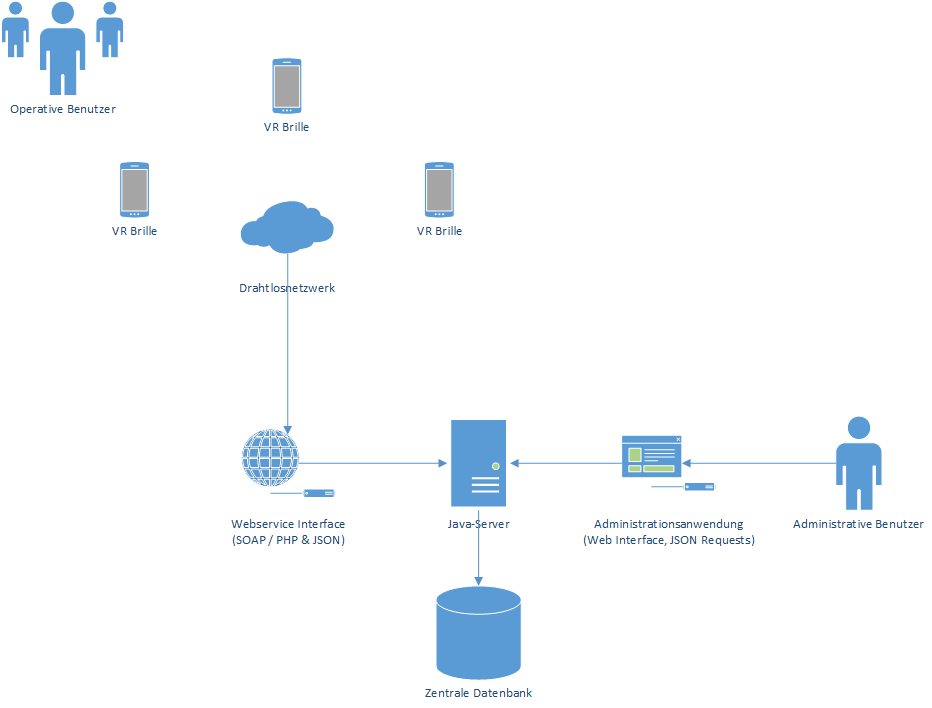
\includegraphics[width=\textwidth]{Bilder/Abbildungen/architektur_serverclient.png}}
	\caption{Schematische Darstellung der Server-Client-Architektur}
	\label{fig:architektur_serverclient}
\end{figure}

Im Folgenden werden die einzelnen Akteure mit ihren jeweiligen Komponenten genauer beschrieben.

\subsection{Server}

Der Server ist logisch in drei Komponenten unterteilt: einen Datenbankserver, einen Webserver mit Web-Interface und Client-Schnittstelle. Diese Komponenten müssen nicht zwingend auf dem selben Server \bzw auf dem selben Gerät installiert sein -- es kann es Sinn machen, ressourcenintensive Anwendungen auf weitere Geräte auszulagern. Gäbe es zum Beispiel sehr viele Clients, die viel Netzwerktraffic über die REST API erzeugen, wäre eine Auslagerung der API auf einen separaten Server bzw. Serverprozess denkbar, um die Performance der anderen Anwendungen nicht zu verringern. Ebenso wäre eine Auslagerung der Datenbank oder des Web-Interface möglich.

Der Einfachheit halber wird bei den folgenden Erläuterungen in dieser Arbeit davon ausgegangen, dass alle Komponenten auf dem selben Server liegen.

\subsubsection{Datenbankserver}
Der Datenbankserver (auch \ac{DBMS}) bildet die Kommunikationsschnittstelle, über die alle Anwendungen auf die Datenbank zugreifen. Die Datenbank selbst ist eine relationale \acs{SQL}-Datenbank, auf welche als \ac{DBMS} MySQL aufgesetzt wurde. Diese Entscheidung liegt darin begründet, dass für das Web-Interface und die REST API als serverseitige Scriptsprache \acs{PHP} gewählt wurde und dazu üblicherweise MySQL als DBMS verwendet wird, aufgrund der guten Kompatibilität und Bewährtheit.

\subsubsection{Web-Interface}
Das Web-Interface bildet die Administrationsoberfläche, über die das System gesteuert werden kann. Hier können die Benutzer des Systems und ihre Berechtigungen verwaltet werden. Außerdem bietet die Webadministration umfangreiche Möglichkeiten, um die Entitäten des Systems zu konfigurieren, wie z.B. Produkte oder Regale auf der Verkaufsfläche.

\subsubsection{Client-Schnittstelle}
Damit die Clients Daten aus der Datenbank abfragen oder ändern können, wird eine weitere Systemschnittstelle benötigt -- die Verwendung der Webadministration zur Datenmanipulation, z.B. über die Datenbrille, ist aus ergonomischen Gründen nicht geeignet, da die Brille nur eingeschränkte Eingabemöglichkeiten hat und ohnehin über eine eigens entwickelte App mit Zusatzfunktionen wie z.B. Barcode-Scanner verfügt.

Die Schnittstelle stellt Dienste für alle Funktionen bereit, die von den Clients benötigt werden, z.B. einen Dienst zum Abruf von Produktinformationen, oder einen Dienst zum Aktualisieren des Warenbestandes. Das Kommunikationsverfahren und die bereitgestellten Dienste werden im Implementierungsteil dieser Arbeit erläutert.

\subsection{Clients}
Wie bereits in der Einführung der Architektur angedeutet, handelt es sich bei den Clients im System von \acs{SMAR} um alle Geräte, die von operativen Benutzern im System verwendet werden: z.B. Smartphones, Tablets und -- im Fall dieser Arbeit mit besonderem Fokus -- Datenbrillen. Diese Geräte kommunizieren über das Netzwerk mit der \acs{REST} \acs{API}, um Lese- und Schreibzugriffe auf den Daten auszuführen.

\section{Datenbank-Architektur}
\label{sec:architektur_datenbank}

Der Entwurf der Datenbank erfordert besonders sorgsame Planung. Das Datenbankschema sollte künftige Erweiterungen der Software unterstützen und späteren Anpassungen am Schema möglichst vorbeugen, da sowohl das Web-Interface als auch die \acs{REST} \acs{API} auf dem Schema arbeiten und somit bei Änderung des Schemas auch weitreichende Änderungen im Quellcode die Folge wären (Anmerkung: für die App auf der Brille oder anderen Clients wären durch die Abstraktion über die \acs{REST} \acs{API} u.U. keine Anpassungen nötig).\\
Deshalb wurden bei der Planung der Datenbank für SMAR bereits Funktionen berücksichtigt, die in der dieser Arbeit zugrunde liegenden Version noch nicht implementiert sind, und entsprechende Tabellen und Spalten angelegt. Die grafische Übersicht veranschaulicht das Schema mit allen Tabellen, Spalten und Beziehungen von Feldern untereinander und wird im Folgenden näher erläutert (größere Version im Anhang):

\begin{figure}[H]
	\centering
	{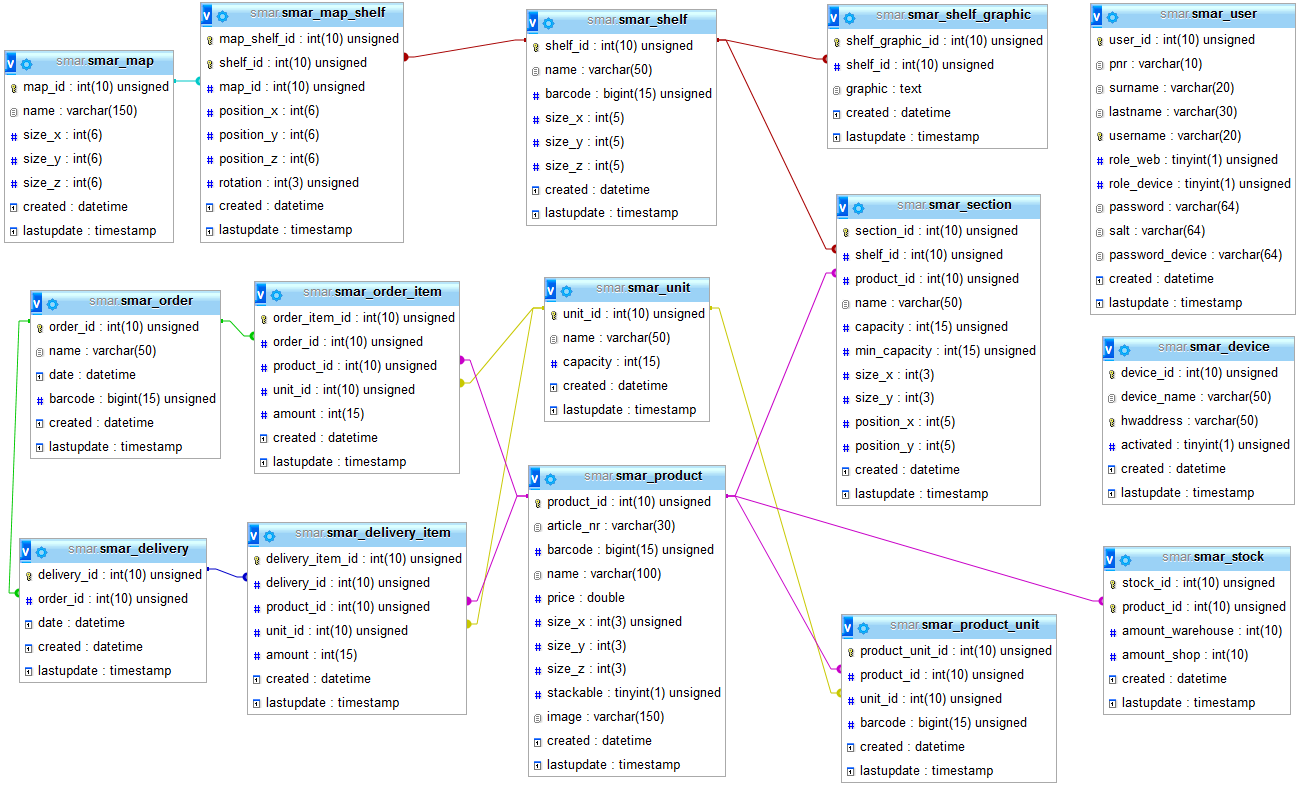
\includegraphics[width=\textwidth]{Bilder/Abbildungen/architektur_datenbankschema.png}}
	\caption{Tabellendefinitionen der MySQL-Datenbank (Screenshot aus phpMyAdmin)}
	\label{fig:architektur_datenbankschema}
\end{figure}

Im Shelf-Management drehen sich die grundlegenden Prozesse um Produkte -- dementsprechend gehört die Tabelle \textit{\textbf{product}} zu den umfangreichsten Tabellen. Hier werden alle wesentlichen Informationen zu einem Produkt gespeichert, z.B. Bezeichnung, Artikelnummer und Preis. Wichtig ist auch der abgespeicherte Barcode, über den das Produkt beim Scannen über die Brille identifiziert werden kann. Außerdem können die Maße des Produktes (Höhe, Breite, Tiefe) sowie die Stapelbarkeit (ja oder nein) angegeben werden -- diese Daten können bei der Lagerplatzberechnung interessant sein.\\

Mit der Tabelle \textit{\textbf{product}} sind weitere Tabellen logisch verknüpft. Sehr wichtig im Rahmen des Shelf-Managements ist der Lagerbestand eines Produktes, welcher in der Tabelle \textit{\textbf{stock}} gespeichert wird. Konzeptionell ließe sich der Warenbestand direkt in \textit{\textbf{product}} speichern -- aus Gründen der Übersichtlichkeit und Performanz wurde die Speicherung vom Produkt logisch getrennt, da die Schreib- und Lesezugriffe auf den Warenbestand in der Anwendung oft isoliert erfolgen. Es können mehrere Bestände für ein Produkt erfasst werden: Bestand im Lager der Filiale (\textit{amount\_warehouse}) und Bestand im Regal bzw. auf der Verkaufsfläche (\textit{amount\_shop}). Diese Bestände werden entsprechend bei der Warenannahme, beim Einräumen in das Regal sowie an der Kasse beim Verkauf verändert. Prinzipiell können hier auch weitere Lagerorte hinzugefügt werden.\\

Produkte werden im Lager und im Shelf-Management oft nicht nur einzeln, sondern auch in bestimmten größeren Mengen prozessiert, bspw. in Form von Kartons fester Größe; Produkte werden i.d.R. karton- oder sogar palettenweise bestellt und oft auch kartonweise auf der Verkaufsfläche eingeräumt. Für diesen Anwendungsfall können feste Produkteinheiten (\glqq units\grqq ) in der Tabelle \textit{\textbf{unit}} definiert werden. Die Beziehung zwischen einer Einheit und einem Produkt wird in \textit{\textbf{product\_unit}} beschrieben. Diese Trennung der Produkt-Einheit-Beziehung ermöglicht eine Wiederverwendbarkeit von Produkteinheiten für mehrere Produkte. Jeder Produkt-Einheit-Beziehung kann ein eigener Barcode zugewiesen werden, sodass bspw. ein entsprechender Karton beim Scannen mit der Brille direkt erkannt werden kann.\\

Die Verwendung von Produkteinheiten ist grundsätzlich optional, da diese über Zusatzfunktionen der Software bzw. einen separaten Barcode angesprochen werden. Je nach Umsetzung im Handel haben z.B. Kartons entweder einen eigenen Barcode, oder den selben Barcode wie das Produkt, oder gar keinen Barcode; alle diese Fälle lassen sich mit diesem Datenbankschema abbilden und nutzen.\\

Neben dem Produkt ist das Verkaufsregal eine weitere wesentliche Entität im Shelf-Management. Regale werden über die Tabelle \textit{\textbf{shelf}} definiert, haben eine feste Größe (Höhe, Breite, Tiefe) und können ebenfalls über einen Barcode identifiziert werden.\\

Die Verbindung zwischen Regalen und Produkten bilden die Regalfächer (\glqq sections\grqq ) in der Tabelle \textit{\textbf{section}}. Ein Regalfach wird genau einem Regal zugeordnet und kann genau einen Produkttyp aufnehmen. Es werden die Größe des Fachs (Breite, Höhe) sowie die Position des Fachs im zugeordneten Regal (Abstand zu linker oberer Ecke als X/Y Koordinaten) abgespeichert. Außerdem ist die maximale Kapazität des Regalplatzes angegeben (also die höchstmögliche Befüllung mit dem zugeordneten Produkt), sowie optional ein Mindestfüllbestand. Letzterer kann verwendet werden, um im System anzuzeigen, welche Produkte aufgefüllt werden müssen, damit die entsprechenden Regalfächer nicht komplett leer werden.\\

Mit der Tabelle  \textit{\textbf{shelf}} sind ebenfalls noch weitere Tabellen verbunden. Die Tabelle  \textit{\textbf{shelf\_graphic}} speichert vorgenerierte Grafiken der Regale im \ac{SVG}-Format, die von der App auf der Brille direkt verwendet werden können, um Rechenaufwand zu sparen. Um eine Wegfindung zu Regalen auf der Verkaufsfläche realisieren zu können, können in der Tabelle \textit{\textbf{map}} Verkaufsflächen definiert werden, sowie über die Tabelle \textit{\textbf{map\_shelf}} Regale auf einer Verkaufsfläche angeordnet werden.\\

Um bei der Warenannahme die erhaltene Ware mit vorausgegangenen Bestellungen abgleichen zu können, müssen die Bestellungen im System hinterlegt sein. In der Tabelle \textit{\textbf{order}} können einzelne Bestellungen gespeichert werden, die zugehörigen Positionen liegen in der Tabelle \textit{\textbf{order\_item}}, welche wiederum auf Entitäten der Tabellen  \textit{\textbf{product}} und \textit{\textbf{unit}} verweist.\\
Mit der selben Struktur sind die Tabellen \textbf{\textit{delivery}} und \textit{\textbf{delivery\_item}} aufgebaut. Diese dienen dazu, die bei der Warenannahme erfassten Produkte und Mengen einer Lieferung zu speichern, damit aus der tatsächlichen Lieferung im Abgleich mit der Bestellung aus der Tabelle \textit{\textbf{order}} eine Differenzliste erstellt werden kann.\\

Im System von \acs{SMAR} können in der Praxis sehr viele Client-Geräte eingebunden sein, welche im Shelf-Management eingesetzt werden. Um diese Geräte zu verwalten, werden alle wesentlichen Geräteinformationen (\zB Hardware-Adresse und Zugriffsberechtigung) in der Tabelle \textit{\textbf{device}} gespeichert.\\

Zuletzt sei auch die Tabelle \textit{\textbf{user}} genannt, welche wesentlich für die Sicherheit der Anwendung ist. Sie speichert alle Informationen zu den Benutzern des Systems: die Basisdaten zu einer Person, die Zugangsdaten für das Web-Interface und die Smartglass, sowie die jeweils zugeordneten Berechtigungen eines Benutzers.\\


\chapter{\acs{PHP} \acs{JWT}}
\label{cha:jwt}
\sloppy

Bei der in diesem Projekt genutzten Bibliotek \glqq PHP JWT\grqq\ handelt es sich um eine objektorientierte \ac{PHP}-Klasse von \mbox{\url{firebase.com}} zur Generierung von \acl{JWT}.
\fussy
\begin{figure}[H]
	\centering
	{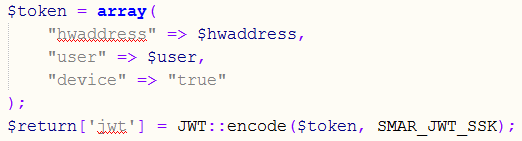
\includegraphics[scale=1.0]{Bilder/jwt_encode.png}}
	\caption{Generierung eines \acs{JWT}}
	\label{fig:jwt_encode}
\end{figure}

Abbildung \ref{fig:jwt_encode} zeigt die Generierung eines \ac{JWT}. \$token beschreibt dabei das \ac{JSON}-Objekt und enthält den Inhalt. SMAR\_JWT\_SSK ist eine in der Konfigurationsdatei festgelegte Konstante und beschreibt den Secret Server Key (geheimer Schlüssel), der nur dem Server bekannt ist, anhand dessen der Inhalt signiert wird. Dadurch wird sichergestellt, dass der \ac{JWT} bei einer weiteren Anfrage an den Server nicht durch den Client manipuliert wurde.\\

Die Dekodierung eines solchen \acl{JWT} wird in Abbildung \ref{fig:jwt_decode} beschrieben. Dabei muss SMAR\_JWT\_SSK (Secret Server Key) identisch zu dem Schlüssel sein, der zur Generierung des \ac{JWT} benutzt wurde. Sind die Schlüssel nicht identisch, wird der Token nicht dekodiert und die Funktion liefert ein leeres Ergebnis zurück.

\begin{figure}[H]
	\centering
	{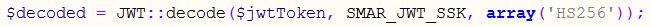
\includegraphics[scale=1.0]{Bilder/jwt_decode.png}}
	\caption{Dekodieren eines \acs{JWT}}
	\label{fig:jwt_decode}
\end{figure}

Ein \ac{JSON} Web Token setzt sich aus folgenden drei Abschnitten zusammen:\footnote{\citep[S. 289f.]{book_jwt}}
\begin{enumerate}
	\item JSON-Objekt, welches den \acs{JWT}-Header repräsentiert
	\item JSON-Objekt bestehend aus verschiedenen Name/Wert-Paaren (Claims-Set), welche die Daten des Benutzers enthält, in diesem Projekt \zB:
	\begin{itemize}
		\item die \acs{MAC}-Adresse des Gerätes und
		\item den Benutzernamen des angemeldeten Benutzers
	\end{itemize}
	\item die Signatur
\end{enumerate}
Alle drei Abschnitte sind jeweils mit BASE64-codiert und werden durch einen Punkt (.) voneinander getrennt.\\

Der \acs{JWT}-Header besteht ebenfalls aus zwei Name/Wert-Paaren und sieht in diesem Projekt wie folgt aus:
\begin{figure}[H]
	\centering
	{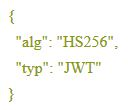
\includegraphics[scale=1.0]{Bilder/jwt_header.jpg}}
	\caption{\acs{JWT}-Header}
	\label{fig:jwt_header}
\end{figure}
Der Header beschreibt den Typ (JWT) und den verwendeten Algorithmus \shorthandoff{"} ("alg":"HS256") \shorthandon{"} zur Signierung. In \ac{SMAR} wurde der HS256-Algorithmus zur Signierung des Claims-Set verwendet. Das Claims-Set wurde somit mit einem privaten Schlüssel und SHA-256 zu einem Hash-Wert errechnet (dies ist der dritte Teil des \acs{JWT}). Die Signierung kann aufgrund des symmetrischen Signierungsalgorithmus außerdem nur mit dem selben privaten Schlüssel überprüft werden.\\
Ein \acl{JWT} stellt somit die Identität der Nachricht \bzw des \ac{JSON}-Objekt sicher und verhindert die unbemerkte Manipulation.\\

Durch den Einsatz von PHP JWT wird in \ac{SMAR} die korrekt authentifizierte Kommunikation mit der REST API - sowohl von der App, als auch von der Web Administration - sichergestellt.
Mit der Anmeldung an der Brille \bzw an der Weboberfläche wird eine Authentifizierungsanfrage an den Server (Web Administration) oder an die REST Api (\acs{VR}-Gerät) gestellt, ist die \acl{AuthN} erfolgreich, so wird ein gültiger \ac{JWT} mit Hilfe der PHP JWT-Klasse generiert. Dieser wird an die PHP-Session in der Web Administration oder an das \acs{VR}-Gerät zurückgegeben. Bei einer Anfrage an die REST Api muss dieser \acs{JWT} mitgegeben werden. Die REST Api dekodiert bei einer Anfrage zunächst den Token mit PHP JWT. Ist die Signatur gültig, wird ein JSON-Objekt zurückgegeben, ansonsten gibt es nur eine leere Antwort. Anschließend werden die Daten des JSON-Objekts mit der Datenbank verglichen, dies stellt sicher, dass die Berechtigung zur Ausführung noch vorhanden ist. Ist auch dies Erfolgreich wird die Anfrage ausgeführt. Bei einem Fehlerfall wird die Anfrage mit einer Fehlermeldung revidiert.
\chapter{Rechteverwaltung - Web}
\label{cha:rechteverwaltung_web}
Die Web Administration stellt die zentrale Kontrolleinheit des gesamten Projekts dar. Über die Web Administration werden sämtliche Einträge der Datenbank verwaltet, dies schließt neben der Benutzer- und Geräteverwaltung ebenfalls die Verwaltung aller Regale und Produkte ein.\\
Dies sollte selbstverständlich ausschließlich durch autorisierte Personen durchführbar sein.\\

Die folgenden Kapitel befassen sich mit der Identifikation (\acs{AuthN}) und mit der Berechtigungskontrolle (\acs{AuthZ}) eines Benutzers gegenüber dem Webserver.

\section{\acf{AuthN}}
Ruft ein Benutzer eine URL der Webadministration auf, so wird zunächst überprüft, ob bereits eine mit Inhalt gefüllte \ac{PHP}-Session besteht, ist dies nicht der Fall wird der Benutzer auf die Login-Seite weitergeleitet. Der Benutzer hat nicht die Möglichkeit ohne \acl{AuthN} auf die Startseite oder eine Unterseite der Anwendung zu gelangen. Dementsprechend können ebenfalls keine Funktionen aufgerufen werden.\\
Ein Zugriff auf die \ac{REST} \ac{API} ist ohne Anmeldung ebenfalls nicht möglich, da der \ac{JWT} erst bei der Anmeldung generiert wird und Anfragen ohne gültigen \ac{JWT} abgebrochen werden.\\

Die Login-Seite hält ein \ac{HTML}-Formular mit zwei Eingabe-Feldern bereit, die die Eingabe des Benutzernamens und des Passworts ermöglichen. Diese Daten werden durch Absenden des Formulars an ein \ac{PHP}-Skript auf dem Server verschickt. Dieses Skript ruft den Eintrag der Datenbank ab, bei dem der Benutzername mit dem eingegebenen Namen identisch ist. Dem eingegebenen Passwort wird anschließend der Salt-Wert, der dem Benutzer in der Datenbank zugeordnet ist, angehängt und das zusammengesetzte Passwort wird mit dem SHA256-Verfahren gehasht. Das Passwort in der Datenbank wurde ebenfalls mit dem selben Verfahren gehasht und sollte daher identisch mit dem gehashten eingegebenen Passwort sein. Hat die Anfrage nach dem Benutzernamen einen Eintrag zurückgeliefert und die gehashten Passwörter sind identisch, so war der Login erfolgreich.\\
Bei einem erfolgreichen Login werden anschließend folgende Daten in einer neu erstellten \ac{PHP}-Session gespeichert:
\begin{itemize}
	\item Benutzer-ID (Primary Key der Datenbank)
	\item Benutzername
	\item Vorname
	\item Nachname
	\item gehashtes Password
	\item Personalnummer
	\item Berechtigungsstufe
	\item Loginzeit (Datum + Uhrzeit)
	\item Zeit seit dem letzten Seitenaufruf (Datum + Uhrzeit)
	\item ein gültiger \ac{JWT} zur Authentifizierung gegenüber der \ac{REST} \ac{API}\footnote{Siehe Kapitel \ref{cha:jwt} \nameref{cha:jwt}}
\end{itemize}
Der \ac{JWT} wird im Rahmen der der Session-Erstellung generiert.\\
Nach Generierung der Session wird nun die Startseite der Anwendung angezeigt.\\
Sollte der Login-Vorgang aufgrund einer ungültigen Benutzername/Passwort-Kombination so wird die Login-Seite mit einer entsprechenden Fehlermeldung erneut angezeigt.\\

Das Hash-Verfahren für das Passwort, so wie ein individueller Salt-Wert pro Benutzer stellen eine Authentifizierung nach aktuellem Standard mit hoher Sicherheit dar. Auch wenn einem Angreifer das Auslesen der Benutzerdaten aus der Datenbank gelingt, kann er das Passwort eines Benutzers und somit den Zugriff mit einer vorgefertigten Rainbowtabelle nicht erlangen. Er muss eine große, für jeden Benutzer individuelle Rainbowtabelle anlegen, die bei einer Passwortlänge von mindestens 64 Zeichen (Salt-Wert-Länge) bei mindestens 52 möglichen Zeichen (A-Z und a-z) mehrere hundert Terabyte groß ist.\footnote{TODO: Rechnung}\\

TODO:
\begin{itemize}
	\item Session-Überprüfung/Aufrufen weiterer Seiten bei Anmeldung
	\item REST Api?
	\item Benutzerverwaltung erklären
\end{itemize}

\section{\acf{AuthZ}}
Im Gegensatz zu den Benutzern der \ac{VR}-Geräte, die entweder durch ihre Aufgabe volle Berechtigung auf den \ac{AR}-Geräten oder keine Berechtigung benötigen und es somit keine verschiedene Berechtigungsstufen benötigt, gibt es in der Web Administration verschiedenste Benutzern mit unterschiedlichen Berechtigungen im Unternehmen.\\
Während der Filialleiter sowohl Zugriff auf die Benutzerverwaltung, als auch auf die Regal- und Produktverwaltung haben sollte, so sollte ein Mitarbeiter, der für die Warenannahme und -einräumung beauftragt wurde, keinen Zugriff auf die Benutzerverwaltung haben.\\
Vor Allem durch die Benutzerverwaltung ist hier ebenfalls auf rechtliche Bestimmungen zu achten. § 3a Satz 2 \acs{BDSG}\footnote{\acf{BDSG}}:
\begin{quote}
	\glqq \textit{Die Erhebung, Verarbeitung und Nutzung personenbezogener Daten und die Auswahl und Gestaltung von Datenverarbeitungssystemen sind an dem Ziel auszurichten, so wenig personenbezogene Daten wie möglich zu erheben, zu verarbeiten oder zu nutzen. Insbesondere sind personenbezogene Daten zu anonymisieren oder zu pseudonymisieren, soweit dies nach dem Verwendungszweck möglich ist und keinen im Verhältnis zu dem angestrebten Schutzzweck unverhältnismäßigen Aufwand erfordert.}\grqq
\end{quote}
sagt aus, dass auch die Nutzung von personenbezogenen Daten, wie sie in der Benutzerverwaltung abgespeichert werden müssen, so weit wie möglich reduziert werden soll. Ein Mitarbeiter, der nicht im Personalmanagement angestellt oder mit Aufgaben der Benutzerverwaltung beauftragt ist, sollte somit auch keinen Zugriff auf personenbezogene Daten haben. Im Zweifelsfall wäre dieser Benutzer eventuell sogar unberechtigt diese Daten einzusehen.\\

Die Autorisierung von Benutzern konnte in \ac{SMAR} dahingehend vereinfacht werden, dass davon ausgegangen wurde, dass die verschiedenen Berechtigungsstufen aufeinander aufbauend sind. Das heißt jemand in einer höheren Berechtigungsstufe hat immer die Berechtigungen der darunterliegenden Berechtigungsstufe und darauf aufbauende Rechte. Eine niedrigere Berechtigungsstufe hat somit niemals Rechte, die eine höhere Stufe nicht besitzt.\\

Aus den Aufgaben dieses Projektes und der Berücksichtigung eventueller Gesetzesvorgaben ließen sich die folgenden acht Berechtigungsstufen herleiten:
%\begin{enumerate}
%	\item[0]: keine Berechtigung
%	\item[10]: Products, Units, Shelves, Sections lesen; keine Schreibberechtigung
%	\item[20]: Schreibberechtigung für Products \& Units
%	\item[30]: Schreibberechtigung für Bestellungen
%	\item[40]: Schreibberechtigung für Products, Units, Shelves \& Sections
%	\item[50]: Lese- und Schreibberechtigung für Geräteverwaltung
%	\item[60]: Lese- und Schreibberechtigung für die Benutzerverwaltung
%	\item[70]: Vollständige Berechtigung
%\end{enumerate}
\begin{figure}[H]
	\centering
	{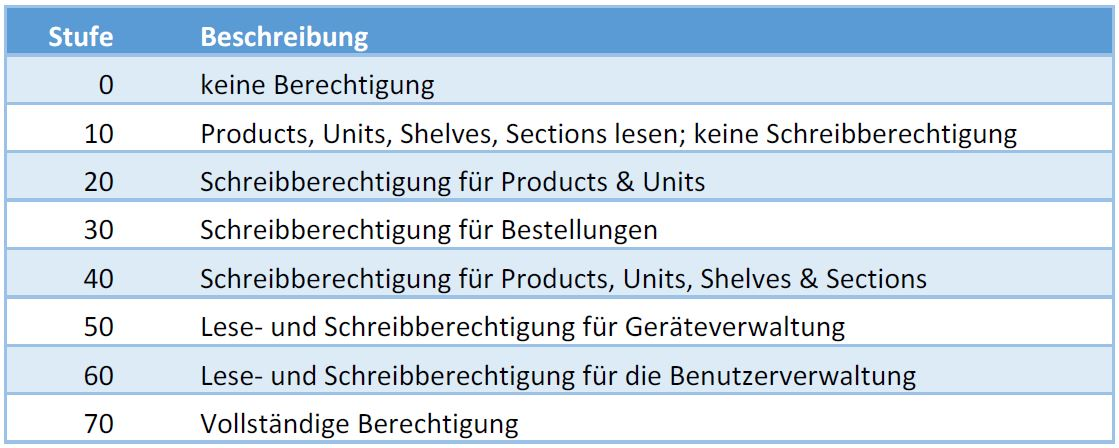
\includegraphics[scale=0.5]{Bilder/role_web.jpg}}
	\caption{Berechtigungsstufen in der Web-Administration}
	\label{fig:role_web}
\end{figure}
Wie im vorherigen Absatz beschrieben, besitzen höhere Berechtigungsstufen automatisch auch die Berechtigungen geringerer Stufen. Außerdem wurde darauf geachtet, dass späteres Erweitern der Funktionalität der Anwendung noch weitere Berechtigungsstufen erfordern könnten. Berechtigungsstufen wurden in Zehnerschritten durchnummeriert, einzelne Berechtigungsstufen können durch Nutzen der Einerschritte in vorhandene Stufen integriert werden ohne dass die Anwendung in bestehenden Programmteilen angepasst werden muss.\\

Berechtigungsstufe 0 gibt dem Benutzer keine Berechtigung die Anwendung zu benutzen, der Anmeldebildschirm wird nicht auf die Startseite weitergeleitet, sondern gibt eine Fehlermeldung \glqq Insufficient Permissions\grqq\footnote{zu Deutsch: \glqq mangelnde Berechtigung\grqq} zurück. Dies kann erforderlich sein, wenn einem Mitarbeiter gekündigt wurde, er aber aufgrund von \zB offenen Gehaltszahlungen noch nicht aus dem System gelöscht werden darf. Berechtigungsstufe 10 gibt Zugriff auf die Anwendung und auf die Basisfunktionalität, der Benutzer bekommt allerdings noch keine Schreibberechtigung. Dies ist für Mitarbeiter sinnvoll, die mit der Überwachung des Warenbestands beauftragt wurden, allerdings keine Berechtigung haben sollen, diesen zu verändern. Die darauffolgende Stufe 20 gibt dem Benutzer zusätzlich die Berechtigung auf die Produktverwaltung. Der Benutzer ist daher berechtigt Produkte zu verändern/hinzuzufügen oder zu löschen. Die Regalverwaltung ist hier noch nicht inbegriffen und wird erst in der Stufe 40 hinzugefügt. Dem Benutzer ist es nun erlaubt Regale, Regalstandorte und die Anordnung der Produkte innerhalb des Regales zu verändern. Darauffolgende Berechtigungsstufen 50, 60 und 70 dienen der Verwaltung und sind für die eigentliche Aufgabenerfüllung nicht mehr notwendig. Stufe 50 fügt die Berechtigung zur Geräteverwaltung hinzu, das heißt der Benutzer darf nun \ac{AR}-Geräte, wie \zB die Smartglass hinzufügen oder löschen. Stufe 60 fügt eine nach dem Gesetz sensible Berechtigung hinzu, nämlich den Lese- und Schreibzugriff auf personenbezogene Daten. Der Benutzer ist nun berechtigt andere Benutzer hinzuzufügen, zu löschen oder zu verändern (wie \zB Berechtigungen verändern). Das Ändern des Passworts des eigenen, angemeldeten Benutzers ist jedoch bereits ab Berechtigungsstufen größer als 0 verfügbar. Die letzte Stufe 70 gewährt volle Berechtigungen auf alle Komponenten der Web-Administration. Dies ist für Systemadministratoren und Filialleiter geeignet, in diesen Fällen muss ein ständiger Zugriff auf die gesamte Anwendung garantiert sein.\\

Die oben genannten Berechtigungsstufen werden in der Datenbank in der für die Benutzer zuständigen Tabelle (user\footnote{Siehe Kapitel \ref{sec:architektur_datenbank} \nameref{sec:architektur_datenbank}}) abgespeichert. Die Tabelle enthält die Spalte role\_web. In dieser Spalte wird für jeden Benutzer die entsprechende Berechtigungsstufe als zweistellige Nummer gespeichert. Greift der Benutzer nun auf die Anwendung zu, wird während der Anmeldung zunächst überprüft, ob die Berechtigung ungleich 0 (keine Berechtigung) ist und anschließend die Berechtigung in der Session gespeichert. Ruft man eine Komponente/eine Funktion innerhalb der Anwendung auf, so wird überprüft, ob die Berechtigungsstufe größer oder gleich (>=) der erforderlichen Nummer ist. Ist die Nummer größer oder gleich wird der Zugang gewährt und die Funktion aufgerufen, ansonsten wird die Anfrage mit der Fehlermeldung \glqq Insufficient Permissions\grqq\footnote{\glqq mangelnde Berechtigung\grqq} abgebrochen.\\
\chapter{Rechteverwaltung - App auf Brille}
\label{cha:rechteverwaltung_vr}



\section{\acf{AuthN}}
Das folgende Kapitel beschäftigt sich mit der Authentifizierung in der App gegenüber dem Server. Benutzte Bibliotheken und Eingabemethoden werden erklärt. Darüber hinaus wird die verwendete Methode mit anderen technisch möglichen Eingabemethoden verglichen.\\

\acl{AuthN} dient der Identifikation einer Person/eines Gerätes.

\subsection{\acs{AuthN} gegenüber der Brille}
Die App auf der eingesetzten Vuzix M100 Virtual Reality Brille wird, wie beschrieben, zur Warenannahme, sowie zum Einräumen von Produkten verwendet - mit der Brille kann der Warenbestand daher aktiv verändert und manipuliert werden.\\
Diese Veränderung sollte, um \zB strukturierten Diebstahl zu vermeiden, nur durch Authentifizierte \acs{AuthN} und Autorisierte \acs{AuthZ} Personen durchgeführt werden.\\

Die gängige Ein-Faktor-Authentifizierung besteht aus der Kombination eines Benutzernamens mit einem Passwort. Dieses Verfahren hat sich bewährt und bietet bei korrekter Implementation eine durchschnittliche Sicherheit vor unbefugtem Zugriff. Diese Sicherheit würde im Rahmen dieser Anwendung ausreichen, da der Angreifer neben den Benutzerdaten, ebenfalls Zugriff auf ein Gerät haben muss, welches:
\begin{itemize}
	\item in das Firmennetzwerk eingebunden ist und
	\item gegenüber dem Server authentifiziert\footnote{s. Kapitel \ref{cha:authn_server}\nameref{cha:authn_server}} ist.
\end{itemize}
Eine Zwei-Faktor-Authentifizierung ist somit bereits gegeben, da der Benutzer sowohl Wissen (Benutzername und Passwort) als auch Besitz benötigt (Die authentifizierte \acl{VR}-Brille).\\
Die Grundlage für eine gute Anwendungssicherheit ist somit gegeben.

Die Brille hat, wie im Kapitel \ref{cha:brille}\nameref{cha:brille} beschrieben, folgende Eingabemethoden:
\begin{itemize}
	\item 4 Knöpfe an der Brille zur Navigation durch das Betriebssystem
	\item Sensoren zur Erkennung von Gesten
	\item Mikrofon zur Erkennung von Sprachbefehlen
	\item Kamera mit entsprechenden Bibliotheken zur Erkennung von Bar- und QR-Codes
\end{itemize}
Die, für die oben beschriebene \acf{AuthN} übliche Eingabemethode, die textbasierte Eingabe über eine entsprechende Tastatur ist über die \ac{VR}-Brille ohne zusätzliche Hardware nicht möglich. Zusätzliche Hardware wäre zu dem umständlich und würde die Bedienung des Gerätes erschweren. Die Usability ist bei dieser Eingabemethode nicht gegeben.\\

Die Eingabe der Anmeldedaten muss daher über andere Eingabemethoden stattfinden und wird in 2 Teile unterteilt:
\begin{enumerate}
	\item Eingabe/Auswahl des Benutzernamens
	\item Eingabe des Passworts
\end{enumerate}

Der Benutzername ist - im Gegensatz - zum Passwort zumindest gegenüber den anderen Mitarbeitern, die Zugriff auf die Brille haben, kein Geheimnis und kann Bekannt sein.\\
Die Eingabe des Benutzernamens über ein Sprachkommando gestaltet sich schwierig und als nicht effektiv. Im Rahmen dieser Arbeit wurde ein Test (TODO: Kapitelrefernzierung auf Kapitel mit Test der Spracherkennung) durchgeführt, der die Spracherkennung testete. Dies funktionierte bei vordefinierten Sprachbefehlen und bei wenig Störgeräuschen zufriedenstellend. Für die Eingabe von Benutzernamen ist dies jedoch nicht geeignet, da die Anmeldung sowohl in ruhigen Umgebungen, als auch lauten Filialen schnell funktionieren muss. Darüber hinaus kann die Erkennung von Eigennamen, die eventuell durch verschiedene Sprachen geprägt sind, nicht zuverlässig garantiert werden.\\
Die Entscheidung fiel daher auf eine Liste, die beim Starten der App vom Server abgerufen wird und auf der LogIn-Seite der App angezeigt wird. Der Server liefert eine Liste mit Benutzern zurück, die für die Brille zugelassen sind (TODO: Kapitelreferenzierung - Rechte). Der Benutzer wählt über die Knöpfe an der Brille den Benutzernamen aus der Liste aus und wird anschließend zur Eingabe des gültigen Passworts aufgefordert.\\
Dies garantiert eine, nach den Möglichkeiten der Vuzix M100 gegebenen, zuverlässige und schnelle Anmeldung. Diese Anmeldemethode ist verständlicherweise nur für eine geringe Anzahl an Benutzern (<30) effizient, jedoch wird davon ausgegangen, dass in einem Supermarkt in der Regel nicht mehr als 20 bis 30 Angestellte mit der Warenannahme/-einräumung beauftragt werden.\\

Auch bei der Passworteingabe gibt es ähnliche Probleme, jedoch muss hier darauf geachtet werden, dass Passwörter ausschließlich dem jeweiligen Benutzer (und eventuell dem Systemadministrator) bekannt sein dürfen \bzw nur im Besitz des Benutzers liegen dürfen. Eine Auswahl aus einer Liste und die Eingabe per Spracherkennung sind somit nicht nur aus Sicht der Bedienung, sondern vor Allem aus Sicherheitsgründen nicht praktikabel.\\
Ein Passwort, das auf Gesten basiert, ist aufgrund der geringen Anzahl an Variationen und möglichen Kombinationen ebenfalls nicht sicher.\\
Die Passworteingabe muss daher über die vierte Eingabemöglichkeit getätigt werden: die Eingabe über Barcodes/QR-Codes mit Hilfe der Kamera.\\

Sobald der Benutzer seinen Benutzernamen aus der Liste ausgewählt hat, wird die Kamera, sowie eine Bibliothek zur Erkennung von QR-Codes gestartet. Der Benutzer scannt seinen persönlichen QR-Code, der in einen String mit einer Länge von 64 Zeichen umgewandelt wird. Diese Daten werden an den Server weitergeleitet, der die Anmeldung schließlich bestätigt (bei korrekter Kombination) oder widerruft (bei ungültigen Login-Daten). Bei korrekter Authentifizierung, gibt der Server einen \ac{JWT} zurück, welcher bei einer Anfrage an den Server mitgeschickt werden muss und auf Korrektheit überprüft wird. Bei einem widerrufenen Login erhält die App ausschließlich eine Fehlermeldung, weitere Anfragen werden aufgrund des fehlenden \ac{JWT} nicht ausgeführt.\\

Der QR-Code kann mit Hilfe der Weboberfläche generiert werden oder es kann ein bestehender Code aktiviert werden (TODO: Kapitelreferenz SMAR Web Administration). Der QR-Code kann durch den Benutzer aufbewahrt werden, sollte der Code in unbefugte Hände gelangen, kann ein neuer Code generiert werden. Außerdem ist es möglich vorhandene Codes, wie \zB ein Code auf der persönlichen Firmen-Zugangskarte des Benutzers, zu verwenden.\\

Die benötigte Sicherheit und das Effiziente Anmelden an die Anwendung ist mit dieser Lösung gewährleistet.

\subsection{\acs{AuthN} gegenüber dem Server}
\label{cha:authn_server}
Im letzten Kapitel wurde beschrieben, wie sichergestellt wird, dass sich nur bekannte und authorisierte Benutzer anmelden können. Das dies nicht unbedingt ausreichend ist, verdeutlicht das folgende Szenario:
\begin{itemize}
	\item Ein Angestellter einer Filiale, der mit der Warenannahme beauftragt ist und somit für die Nutzung der Brille freigeschaltet ist, lässt seinen Firmenausweis beim Einräumen in einem öffentlichen Bereich liegen. Auf dem Firmenausweis sind sowohl der vollständige Name, als auch der QR-Code, der für die Authentifizierung genutzt wird, aufgedruckt. Ein Angreifer, der Zugriff auf das System bekommen möchte, entdeckt dies und fotografiert den Firmenausweis ab.
\end{itemize}
Im oben dargestellten Szenario sind die persönlichen Benutzerdaten - ohne Wissen des Opfers - gestohlen worden. Der Angreifer hat zwar keinen Zugriff auf eine im Markt vorhandene \ac{VR}-Brille, aber eventuell ist er im Besitz der App und hat diese auf einem eigenen Android-Gerät installiert. Ist das Firmennetzwerk zusätzlich noch schlecht abgesichert, \zB durch Nutzung des \ac{WEP} Verschlüsselungsprotokolls, so kann sich der Angreifer mit seinem eigenen Android-Gerät und über die Anmeldedaten des Angestellten auf dem Server authentifizieren.\\
Er kann den Warenbestand nun entsprechend manipulieren und der Filiale schaden zufügen.\\

Um dies zu verhindern, wurde eine Zwei-Faktor-Authentifizierung in die Anwendung integriert. Somit muss sich nicht nur der Benutzer, sondern ebenfalls die \ac{VR}-Brille \bzw das benutzte Gerät gegenüber dem Server authentifizieren.\\

Die App liest dazu beim Starten der Anwendung die \ac{MAC}-Adresse des Gerätes aus und speichert diese in der für den Login zuständigen Klasse ab. Sobald sich der Benutzer anmeldet (seinen Benutzernamen ausgewählt hat und den persönlichen QR-Code eingescannt hat), wird die \ac{MAC}-Adresse an die Login-Daten angehängt und eine Anfrage (Ausführen der "authenticate"-Anwendung der REST Api\footnote{s. Kapitel TODO: Kapitelreferenz auf REST Api-Erklärung}) an den Server mit allen Daten (\ac{MAC}-Adresse, Benutzer, Passwort) geschickt. Ist die \ac{MAC}-Adresse gültig, liefert der Server den \ac{JWT}, ansonsten gibt es eine Fehlermeldungen und alle weiteren Anfragen werden abgelehnt.\\

Eine \ac{MAC}-Adresse und somit das dazugehörige Gerät werden durch einen Eintrag in der Datenbank registriert. Für jedes Gerät wird ein Name, sowie die \ac{MAC}-Adresse vergeben und ein Flag gesetzt, ob dieses Gerät aktuell aktiv sein soll. Das registrierte Gerät kann sich somit gegenüber dem Server erfolgreich identifizieren.

\section{\acf{AuthZ}}
Die \acl{AuthZ} beschreibt - im Gegensatz zur \acl{AuthN} - nicht die Identifikation einer Person/eines Gerätes, sondern prüft die Berechtigungen der bereits vorhandenen Identifikation. Für eine \acl{AuthZ} ist daher eine bereits erfolgreiche \acl{AuthN} erforderlich.

Bei der Benutzung der App gibt es sowohl für das Gerät, als auch für den Benutzer ausschließlich 2 Berechtigungsstufen:
\begin{itemize}
	\item Benutzer/Gerät hat die Berechtigung Daten zu lesen/bearbeiten/löschen,
	\item Benutzer/Gerät hat keine Berechtigung auf die Daten zuzugreifen.
\end{itemize}

Die \acl{AuthZ} findet daher zeitgleich zu der \acl{AuthN} statt. Der \ac{JWT} wird ausschließlich bei erfolgreicher Identifikation und Berechtigung zurückgegeben, ansonsten gibt es eine entsprechende Fehlermeldung.\\

Das Gerät autorisiert sich gegenüber dem Server über das Flag, welches bestimmt, ob das Gerät aktuell aktiv sein soll. Ist dieses Flag gesetzt, besitzt dieses Gerät (\zB \acs{VR}-Brille) volle Berechtigung und weitere Anfragen werden bei gültigem \ac{JWT} übergeben, ansonsten werden alle weiteren Anfragen abgelehnt. Diese \acl{AuthZ} macht Sinn, sollte das Gerät kurzfristig nicht in der Filiale sein. Das Gerät kann gesperrt und reaktiviert werden, ohne dass es gelöscht und anschließend wieder registriert werden muss.\\

Da ein Benutzer ebenfalls nur diese zwei Berechtigungsstufen beim Benutzen der App besitzt, wird die Anfrage ähnlich der Brille ausgeführt. Ein Benutzer besitzt in seinem Datenbank-Eintrag in der Spalte \glqq role\_device\grqq~~ entweder eine 1 (true) und wird autorisiert oder eine 0 (false) und der Server meldet einen entsprechenden Fehler zurück.\\

Weitere Berechtigungsstufen werden an dieser Stelle nicht benötigt, da ein Angestellter, der mit der Warenannahme oder -einräumung beauftragt ist, die gesamte App-Funktionalität benutzt und ein Angestellter, der keine der beiden Aufgaben benötigt, keinen Zugriff auf die Brille benötigt.
%\chapter{Hinweise}
%
%Ist die Architektur richtig gewählt?! Node.js für Asynchrone Webaufrufe deutlich besser! Als Anmerkung ins Fazit packen und Auswahl von PHP auf vorhandenes Wissen  schieben!\\
%
%Ausblick: Technik muss besser werden, Schwachstellen in Usability\\
%
%Acronym \acf{CAS}\\
%
%Internet-Source in footnote\footnote{\citep{cas}}\\
%
%Book-Source in footnote\footnote{\citep{einfuehung_sap_hana}}\\
%
%\begin{figure}[H]
%	\centering
%	{
\includegraphics[height=5cm]{Bilder/logo_dhbw_ma.jpg}}
%	\caption{Example of a figure \protect\citep[page 32]{cas}}
%	\label{fig:Example}
%\end{figure}

\chapter{Reflexion}
Das folgende Kapitel beschäftigt sich mit der kritischen Reflexion der Leistung und Entscheidungen des Projektteams und bezieht sich ausschließlich auf die Software.\\

\begin{figure}[H]
	\centering
	{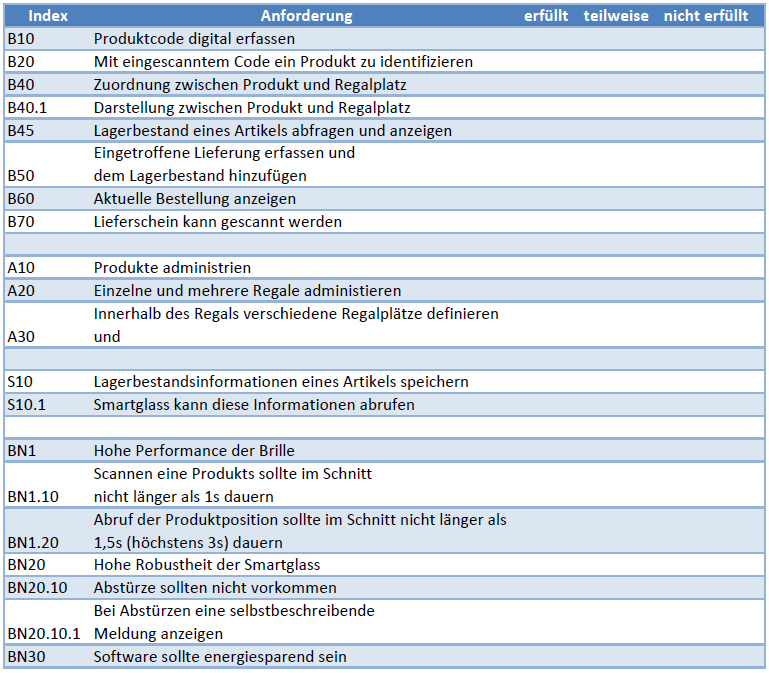
\includegraphics[scale=0.73]{Bilder/Abbildungen/anforderungen_zusammenfassung_bewertung.png}}
	\caption{Übersicht der Anforderungen mit Erfüllungsgrad}
	\label{fig:anforderungen_erfuellt}
\end{figure}

Während die grundlegende Architektur, das Projekt \ac{SMAR} in einer Thin Client-Server-Architektur aufzubauen, in diesem Szenario durchaus Sinn macht, da in der Anwendung mehrere Clients vorhanden sind, die alle auf dieselben Daten - teilweise gleichzeitig - zugreifen, würde eine Berechnung der Daten auf den Clients inkonsistente Stände verursachen und die Performanz negativ beeinflussen. Außerdem waren die eingesetzten Technologien auf den Smartglasses durch das Android Betriebssystem weitestgehend vorgegeben. Entscheidungen wie \zB das Benutzen der ZBar Library, statt der ZXing Anwendung zur Bar-Code-Erkennung sorgen dafür, dass das Projekt eigenständig funktioniert und keine weiteren Softwarevoraussetzungen benötigt. Die \ac{REST} \ac{API} erzeugt eine einfache Kommunikation zwischen Clients (Web Administration und Android-App) und Server und wird von allen Teilen sehr gut unterstützt. Die Web Administration jedoch, die größtenteils eine asynchrone Kommunikation benutzt, kommuniziert im Hintergrund mit PHP-Skripten. Dies ist vor Allem aufgrund der asynchronen Arbeitsweise sehr kompliziert gelöst und nicht zeitgemäß. Hier wäre es von Vorteil gewesen einen NodeJS-Server mit einem AngularJS-Webfrontend einzusetzen. Dies hätte die Programmierung vereinfacht und deutlich Zeit gespart.\\

Das zu Beginn der Entwicklung vereinbarte Zeitmanagement wurde durch das gesamte Projektteam nicht eingehalten. Betrachtet man entsprechende Pushs auf dem Git-Repository sind deutliche Fortschritte zu Anfang des Projekts, zu Anfang des Jahres und zu Ende des Projekts zu verzeichnen. Eine bessere Verteilung und ein kontinuierlicheres Arbeiten am Projekt hätten das Ergebnis verbessern und Schwachstellen in der Architektur und Technologieauswahl frühzeitig aufdecken können.

\chapter{Ausblick}
\label{cha:ausblick}
Im gesamten Projektverlauf wurde sowohl in der Hard- als auch in der Software erkannt, dass sich das Shelf Management mit Wearable Computern noch in einem frühen Stadium befindet. Dennoch kann das Potential hinter dieser Technologie in Verbindung mit dieser Software erkannt werden. Eine Wiederaufnahme des Projekts könnte fehlende oder wünschenswerte Funktionen hinzufügen, die im folgenden als Möglichkeiten erläutert werden sollen.\\

\ac{SMAR} beschäftigt sich, wie der Titel bereits sagt, vor allem auch mit Augmented Reality. Dies wurde im Rahmen dieses Projektes mit Vektorgrafiken dargestellt, die die Realität nachbilden und dem Benutzer eine Orientierung in der realen Welt vermitteln sollen. Durch entsprechende Analysen von Vorschaubildern der integrierten Kamera könnte auf die Darstellung der Regale über Grafiken verzichtet werden. Stattdessen wäre eine Manipulation der Kamerabilder denkbar, in denen die ausgewählte Section eines Regales im Sichtfeld markiert wird. Dies würde dem Benutzer das Übertragen der fiktiven Welt auf die reale Welt ersparen und er könnte sich noch effektiver auf die eigentliche Aufgabe konzentrieren.\\
Die eingebaute Kamera, sowie hauptsächlich das Display müssten jedoch eine deutlich höhere Qualität für ein zufriedenstellendes Ergebnis liefern.\\
Bei Geräten, die eine entsprechende Kamera nicht besitzen oder von der Handhabung nicht für Augmented Reality geeignet sind (wie \zB Smartphones), würden bereits von einer Erweiterung der SVG-Grafiken um Produktbilder am korrekten Regalplatz profitieren. Der Benutzer würde zwar noch nicht das reale Regal sehen, könnte die SVG-Grafiken anhand der realen Produktbilder aber leichter mit der Realität verknüpfen.\\

Im Rahmen dieser Arbeit wurde ausschließlich das Finden der Section innerhalb eines Regales betrachtet. Dies ist für kleinere Einzelhandelsfilialen durchaus ausreichend. Eine Nummerierung der Regale reicht aus, um dem Mitarbeiter die nötigen Informationen für eine effiziente Suche zu geben. Betrachtet man den Großhandel mit großen Lagerhallen und mehreren hunderten Regalen, so wird eine reine Nummerierung nicht mehr reichen, um dem Mitarbeiter das richtige Regal anzuzeigen. Der Mitarbeiter benötigt eine Navigationshilfe. Mit Hilfe von Triangulationsverfahren wäre es möglich eine Indoor-Navigation in \ac{SMAR} zu integrieren. Der Mitarbeiter bekäme so nicht nur den Regalplatz mitgeteilt, sondern eine genaue Navigation auf Grundlage seines Standorts.\\

Im vorgegebenen Zeitrahmen war es darüber hinaus nicht mehr möglich das Android Notification Center in die App einzubinden. Die technischen Voraussetzungen sind gegeben, sodass ein Implementieren der folgenden Funktionalität ohne weitere Librarys möglich wäre. Das Projekt \ac{SMAR} beschäftigt sich mit der Warenannahme und der Wareneinräumung. Dadurch müssen die Lager- und Regalbestände dem Projekt jederzeit bekannt sein. Diese Daten könnte man nutzen, in dem der Benutzer in der App (\zB über das Android Notification Center) benachrichtigt wird, sobald der Regalbestand eine untere Grenze unterschreitet \bzw eine E-Mail an den zuständigen Mitarbeiter versendet wird, sobald der Lagerbestand eine definierte untere Grenze unterschreitet. Unzufriedene Kunden aufgrund von fehlenden Beständen könnten damit zuverlässig verhindert werden. Neben den technischen Voraussetzungen sind die Vorbereitungen in der Datenbank und der Web Administration - durch die Definition der unteren Grenze - bereits getroffen. Für den E-Mail-Versand müsste der Anwendung jedoch ein Service, \zB in Form eines Cron-Jobs hinzugefügt werden, welcher die Lagerbestände regelmäßig prüft.\\

Ein weiterer, für die Usability der App entscheidender Faktor ist die Eingabemethode. Aktuell (Stand: Mai 2015) werden die vier Hardwareknöpfe zur Navigation durch das Android Betriebssystem und der \ac{SMAR}-App benutzt. Dies ist oft sehr umständlich und benötigt eine freie Hand. Als Alternative wurde die Spracherkennung bereits in Kapitel \ref{cha:technik} \nameref{cha:technik} genannt, die aufgrund von mangelnder Qualität - vor allem in lauten Umgebungen - allerdings nicht praktikabel war. Zukünftige Versionen von Smartglasses können eine verbesserte Spracherkennung mit Unterstützung der deutschen Sprache beinhalten. Eine Implementation der Spracherkennung in die App könnte die Eingabe erheblich erleichtern und die Effizienz bei Erledigung der Aufgaben nochmals erhöhen.\\
Um darüber hinaus die Augen des Benutzers zu entlasten, wäre außerdem die Nutzung der Android \glqq android.speech.tts.TextToSpeech\grqq -Klasse denkbar. Diese Klasse ermöglicht die Sprachausgabe von eingegebenem Text. Zusatzinformationen, wie \zB der Lagerbestand, könnten durch die Lautsprecher der Smartglasses an den Benutzer übergeben werden. Ein angenehmerer Tragekomfort wäre die Folge, da die Augen durch das kleine und qualitativ niederwertige Display angestrengt werden.\\


%Das folgende Kapitel beschreibt den möglichen Ausblick einer Shelf Management Software in Verbindung mit einer Augmented Reality Smartglass aus Sicht der Projektteilnehmer. \\
%
%Der angezeigte Ausschnitt eines Regals ist bei dieser Software nur sehr schematisch gewesen. Außerdem wurde bereits im vorherigen Verlauf der Arbeit darauf verwiesen, dass es durchaus denkbar ist, und die Architektur darauf ausgelegt ist, die Kamera der Smartglass dauerhaft mitlaufen zu lassen. Mit zusätzlicher Positionsbestimmung in der Filiale und dauerhafter Kommunikation mit dem Server im Backoff ist bestimmt eine noch bessere und genauere Zielführung zu einem Regalplatz möglich. 
%\\
%Aufgrund der schwachen Auflösung der Kamera, ist es erforderlich die entsprechenden Codes sehr nah an die Linse zu halten, was in einem Live-Betrieb die Arbeit eher behindert als bereichert. Mit einer höheren Auflösung ist auch ein erfassen von entfernten Codes denkbar, sodass neben der Position des Mitarbeiter auch die Blickrichtung dessen erfasst werden kann. Dies ist quasi eine weitere Dimension, die zur Berechnung hinzugezogen werden kann und genauere Hilfen ermöglicht. 
%\\
%Durch höhere Auflösungen könnten der Mitarbeiter beim Vorbeigehen Produkte einscannen. Dabei könnte ihm angezeigt werden, dass manche Produkte nicht an diesen Regalplatz gehören, weil sie vom Kunden verlegt wurden, und weggeräumt werden müssen. 
%\\
%Vor allem bei frische Produkten ist es vorstellbar in den Barcode ein entsprechendes Mindesthalbarkeitsdatum einzuprägen. Beim Vorbeigehen könnte dieses eingescannt und angezeigt werden. Bei kritischen Fällen oder sogar Überläufen könnte dieses entsprechend markiert werden, sodass es einfach aus dem Verkauf genommen werden könnte.
%\\
%Außerdem ist es wahrscheinlich ratsam zum Scannen einiger Produkte nicht nur die Smartglass zu verwenden, sondern auch andere externe Komponenten, wie einen Ringscanner oder einen üblichen Handscanner, der über Bluetooth mit der Smartglass kommuniziert. So sind einige Prozesse bzw. Bewegungen natürlicher sowie ergonomischer für den Mitarbeiter. 
%\\
%Weiter in die Zukunft gedacht, ist es vorstellbar, dass nicht nur Mitarbeiter eine Smartglass verwenden, sondern die Kunden selbst. dazu wären natürlich hohe Stückzahlen und ein entsprechend verlässliches sowie benutzerfreundliches System notwendig. Allerdings wäre der Kunde vollkommen autark und könnte ohne jegliche Interaktion mit einem Mitarbeiter seine Einkäufe erledigen. Außerdem ist es denkbar, wenn der Kunde eine Smartglass verwendet, dass diesem mehr Produktinformationen, wie Nährstoffe passend zu seiner Diät, oder weitere dazu passende Produkte, ähnlich wie "Kunden kauften auch diesen Artikel", angezeigt werden könnten. 
%\\

\chapter{Fazit}
Die in den ersten Kapiteln beschriebene durchgeführte Analyse stellt den IST-Zustand in gängigen Einzelhandelsfilialen dar und erkennt Bedarf in der Unterstützung der Warenannahme und -einräumung durch Wearable Computer. Der Vergleich verschiedener Gerätetypen unterstreicht die Entscheidung, diese Unterstützung mit Hilfe von Smartglasses umzusetzen. Eine entsprechende Anforderungsanalyse inklusive Priorisierung der zu erledigenden Aufgaben stellen sicher, dass \ac{SMAR} bereits in diesem Umfang der großen Studienarbeit zu einem Mehrwert in Filialen führen und die Effizienz und Effektivität im Unternehmen steigern können.\\

Zu Beachten ist, dass sowohl die Hardware in Form von Smartglasses, als auch die Software noch in einem frühen Stadium stehen und daher nicht alle Funktionen ausgereift sind und optimal funktionieren. Dies wird \zB durch das Display der Vuzix M100 deutlich, welches oft nicht optimal ausgerichtet ist und kleine Texte nicht deutlich genug auflöst.\\

Erschwert wurde die Entwicklung außerdem durch fehlende Testmöglichkeiten in entsprechenden Einzelhandelsfilialen. Die durchgeführte Umfrage bei Managern von solchen Filialen half bei der Bedarfs- und Anforderungsanalyse, allerdings konnte nicht getestet werden, ob diese korrekt verstanden, umgesetzt wurden und ob dies den Wünschen der Mitarbeiter an eine entsprechende Technologie entspricht.\\

Dennoch wurden die aus den Umfragen interpretierten Anforderungen mit erster Priorität umgesetzt und bieten daher - zumindest theoretisch - eine erfolgreiche Grundlage. Darüber hinaus muss beachtet werden, dass die Umsetzung entsprechender Systeme noch nicht existiert und dies einen ersten Entwurf einer Entwicklung darstellt.\\

\ac{SMAR} ist daher nicht als eine fertige und einsetzbare Software in Unternehmen anzusehen. \ac{SMAR} bietet viel mehr die Grundlage für entsprechende Proof-Of-Concepts gegenüber möglichen Kunden und ist für Demonstrationen sehr gut geeignet. Die weitere Entwicklung der Software erfordert eine Zusammenarbeit mit dem Kunden inklusive entsprechender Testphasen.\\

Wird das Projekt entsprechend dem oben beschriebenen Absatz verstanden, ist es als Erfolg anzusehen.	


% --------------------------------------------------------------------------------------------- 
%                    Literaturverzeichnis ---------------------------------------------------------------------------------------------

% Anhang
\clearpage
\pagenumbering{roman}


\bibliography{Inhalt/bib}
\bibliographystyle{jurabib}
% ---------------------------------------------------------------------------------------------
%                    Anhang ---------------------------------------------------------------------------------------------

\begin{appendix}
\clearpage
\pagenumbering{Roman}						% römische Seitenzahlen für Anhang
\chapter{Anhang}







\end{appendix}


\end{document}
